\documentclass{beamer}
\usepackage{amsmath}
\usepackage{amssymb}
\usepackage{graphics}
\usepackage{booktabs}
\usepackage{multicol}
\usepackage{hyperref}
\usepackage{rotating}
\usepackage{multirow}
\usepackage{subfig}
\usepackage{eurosym,units}
\usepackage{colortbl,color}
\usetheme{material}
\useLightTheme
\usePrimaryRed
\useAccentGreen

\renewcommand{\theenumii}{\alph{\enumii}}
\defbeamertemplate{itemize subitem}{dash}{--}
\defbeamertemplate{itemize subsubitem}{dash}{--}
\setbeamertemplate{itemize item}[circle]
\setbeamertemplate{itemize subitem}[dash]
\setbeamertemplate{itemize subsubitem}[dash]
\setbeamertemplate{enumerate item}{\arabic{enumi}.}
\setbeamertemplate{enumerate subitem}{(\alph{enumii})}
\usefoottemplate{}

%\usecolortheme{owl}
\usepackage{array}
\newcolumntype{P}[1]{>{\centering\arraybackslash}p{#1}}

\newcommand{\indicator}[1]{\mathrm{1}\left\{{#1}\right\}}



\setbeamertemplate{headline}{}
\usenavigationsymbolstemplate{}

\title{\LARGE Econ 2220: Experimental Economics \\ Dynamic Games}
\author{Alistair J. Wilson }
\date{Fall 2018}
\begin{document}
\maketitle

\begin{frame}{Vespa \& Wilson (2019,2020) }
\begin{card}
Connects behavior to the infinitely repeated
games literature.
\end{card}
\begin{card}
Simplest dynamic game we could think of.

\begin{itemize}
\item Two agents, $\mathcal{I}=\left\{ 1,2\right\} $

\begin{itemize}
\item Two actions, $\mathcal{A}_{1}=\mathcal{A}_{2}$\only<1>{$=\left\{ \mbox{Cooperate},\mbox{Defect}\right\}$}\only<2>{$=\left\{ C,D \right\}$}
\item Two states, $\Omega$\only<1>{$=\left\{ \mbox{Low},\mbox{High}\right\}$}\only<2>{$=\left\{ L,H \right\}$} \pause
\end{itemize}
\item Any simpler in any variable and we would not have a dynamic game
\end{itemize}
\end{card}
\end{frame}


\begin{frame}{Fixed across environments}
    \begin{card}
    \begin{itemize}
    \item Infinite time horizon
    \item Two agents: 1,2
    \item Two states: \textcolor{red}{Low}, \textcolor{blue}{High}
    \item Initial state: \textcolor{red}{Low}
    \item Discounting: $\delta=75\%$\pause
    \item Try to hold constant some of the strategic tensions
    \end{itemize}
    \end{card}
\end{frame}

\begin{frame}

    \begin{card}{Experimental Details}
    \begin{itemize}
    \item Three sessions per treatment
    \item 14 subjects per session, EBEL-UCSB
    \item 350 subjects total
    \item Expected earnings: \$18 (between 75-90 minutes)
    \item 15 repetitions of the supergame
    \item Partial block design
    \end{itemize}
    \end{card}
\end{frame}


\begin{frame}{Structure of a session}
\begin{card}
\begin{center}
\begin{tabular}{c|c|c|c|ccc|c|c|c|}
\multicolumn{1}{c}{} & \multicolumn{9}{c}{Cycle}\\ 
\multirow{14}{*}{\begin{turn}{90}
Round
\end{turn}} & \textbf{\tiny{}1} & \textbf{\tiny{}2} & \textbf{\tiny{}3} & \multicolumn{3}{c|}{\textbf{\tiny{}...}} & \textbf{\tiny{}13} & \textbf{\tiny{}14} & \textbf{\tiny{}15}\\ 
\cline{2-10}
 & \textbf{\textcolor{blue}{\tiny{}1}} & \textbf{\textcolor{blue}{\tiny{}1}} & \textbf{\textcolor{blue}{\tiny{}1}} &  &  &  & \textbf{\textcolor{blue}{\tiny{}1}} & \textbf{\textcolor{blue}{\tiny{}1}} & \textbf{\textcolor{blue}{\tiny{}1}}\\ 
 & \textbf{\textcolor{blue}{\tiny{}2}} & \textbf{\textcolor{blue}{\tiny{}2}} & \textbf{\textcolor{blue}{\tiny{}2}} &  &  &  & \textbf{\tiny{}2} & \textbf{\textcolor{blue}{\tiny{}2}} & \textbf{\textcolor{blue}{\tiny{}2}}\\ 
 & \textbf{\textcolor{blue}{\tiny{}3}} & \textbf{\tiny{}3} & \textbf{\textcolor{blue}{\tiny{}3}} &  &  &  & \textbf{\tiny{}3} & \textbf{\textcolor{blue}{\tiny{}3}} & \textbf{\textcolor{blue}{\tiny{}3}}\\ 
 & \textbf{\textcolor{blue}{\tiny{}4}} & \textbf{\tiny{}4} & \textbf{\textcolor{blue}{\tiny{}4}} &  &  &  & \textbf{\tiny{}4} & \textbf{\textcolor{blue}{\tiny{}4}} & \textbf{\textcolor{blue}{\tiny{}4}}\\ 
 & \textbf{\textcolor{blue}{\tiny{}5}} & \textbf{\tiny{}5} & \textbf{\textcolor{blue}{\tiny{}5}} &  &  &  & \textbf{\tiny{}5} & \textbf{\textcolor{blue}{\tiny{}5}} & \textbf{\textcolor{blue}{\tiny{}5}}\\ 
 & \textbf{\textcolor{blue}{\tiny{}6}} &  & \textbf{\textcolor{blue}{\tiny{}6}} &  &  &  &  & \textbf{\textcolor{blue}{\tiny{}6}} & \\ 
 & \textbf{\textcolor{blue}{\tiny{}7}} &  &  &  &  &  &  & \textbf{\textcolor{blue}{\tiny{}7}} & \\ 
 & \textbf{\textcolor{blue}{\tiny{}8}} &  &  &  &  &  &  & \textbf{\textcolor{blue}{\tiny{}8}} & \\ 
\end{tabular}
\end{center}
\end{card}
\end{frame}

\begin{frame}
\begin{card}
\begin{center}
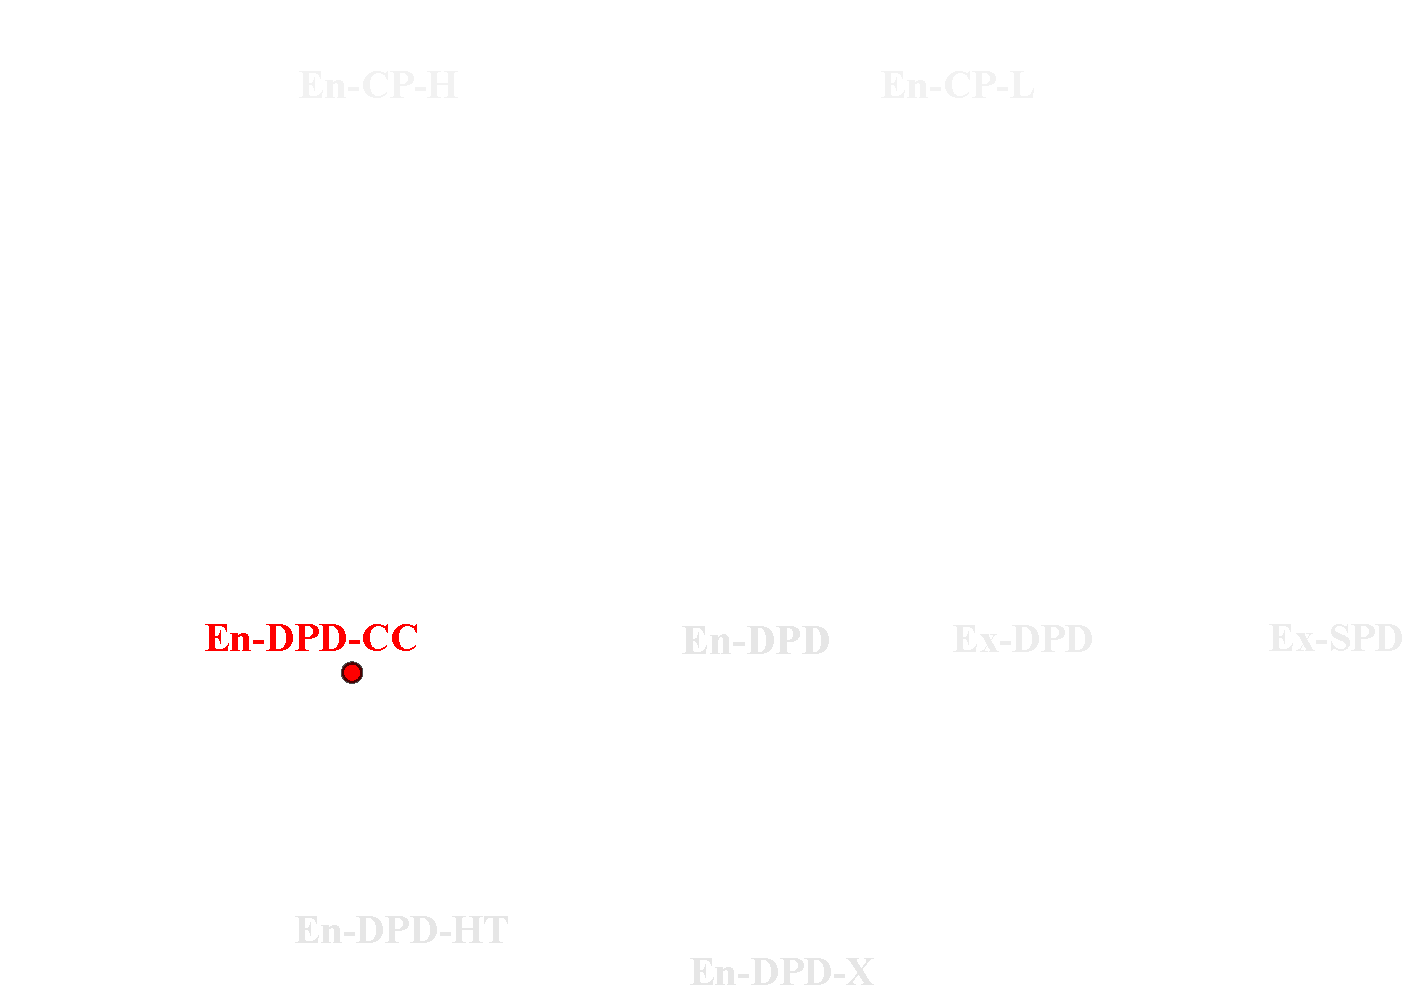
\includegraphics[height=0.7\textwidth]{./i/FlowChart1.pdf}
\end{center}
\end{card}
\end{frame}

\begin{frame}{Endogenous Dynamic PD-CC}

\begin{center}
\begin{table}
\centering{}\subfloat{
\begin{tabular}{ccP{0.14\textwidth}|P{0.14\textwidth}}
\multicolumn{4}{c}{\textcolor{red}{$\omega$=Low}}\\ 
 &  & \multicolumn{2}{c}{2}\\ 
 &  & \multicolumn{1}{P{0.14\textwidth}}{\textbf{C}} & D\\ 
\cline{3-4}
\multirow{2}{*}{1} & \multicolumn{1}{c|}{\textbf{C}} & \small \textcolor{blue}{100,100} & \multicolumn{1}{P{0.14\textwidth}|}{\small \textcolor{red}{30, 125}}\\ 
\cline{3-4}
 & \multicolumn{1}{c|}{D} & \small \textcolor{red}{125, 30} & \multicolumn{1}{P{0.14\textwidth}|}{\small \textcolor{red}{60,60}}\\ 
\cline{3-4}
\end{tabular}}\subfloat{
\begin{tabular}{ccP{0.14\textwidth}|P{0.15\textwidth}}
\multicolumn{4}{c}{\textcolor{blue}{$\omega$=High}}\\ 
 &  & \multicolumn{2}{c}{2}\\ 
 &  & \multicolumn{1}{P{0.14\textwidth}}{C} & \textbf{D}\\ 
\cline{3-4}
\multirow{2}{*}{1} & \multicolumn{1}{c|}{C} & \small \textcolor{blue}{200, 200} & \multicolumn{1}{P{0.15\textwidth}|}{\small \textcolor{blue}{130, 250}}\\ 
\cline{3-4}
 & \multicolumn{1}{c|}{\textbf{D}} & \small \textcolor{blue}{250, 130} & \multicolumn{1}{P{0.15\textwidth}|}{\small \textbf{\textcolor{red}{190, 190}}}\\ 
\cline{3-4}
\end{tabular}}
\end{table}
\end{center}

\begin{card}
\[
\psi\left(\omega ,a \right)=\begin{cases}
\mbox{High} & \mbox{if }a=\left(C,C\right),\omega=\mbox{=Low}\\
\mbox{Low} & \mbox{if }a=\left(D,D\right), \omega=\mbox{\ensuremath{\omega}=High}\\
\omega & \mbox{otherwise}
\end{cases}
\]
\end{card}

\end{frame}


\begin{frame}{Dynamic PD Game CC: Graphical Representation}
\begin{card}
\begin{center}
	\includegraphics<1>[width=0.6\textwidth]{./i/col_GamePayoffs1.pdf}
\end{center}
\end{card}
\end{frame}

\begin{frame}{Endogenous Dynamic PD-CC}
\begin{center}
\begin{table}
\centering{}\subfloat{\centering{}{\small{}}%
\begin{tabular}{ccP{0.1\textwidth}|P{0.1\textwidth}}
\multicolumn{4}{c}{\textcolor{red}{$\omega$=Low}}\\ 

 &  & \multicolumn{2}{c}{2}\\ 
 &  & \multicolumn{1}{P{0.1\textwidth}}{\textbf{C}} & D\\ 
\cline{3-4}
\multirow{2}{*}{1} & \multicolumn{1}{c|}{\textbf{C}} & \textcolor{blue}{100} & \multicolumn{1}{P{0.1\textwidth}|}{\textcolor{red}{30}}\\ 
\cline{3-4}
 & \multicolumn{1}{c|}{D} & \textcolor{red}{125} & \multicolumn{1}{P{0.1\textwidth}|}{\textcolor{red}{60}}\\ 
\cline{3-4}
\end{tabular}
}\subfloat{
\centering{}{\small{}}%
\begin{tabular}{ccP{0.1\textwidth}|P{0.1\textwidth}}
\multicolumn{4}{c}{\textcolor{blue}{$\omega$=High}}\\ 

 &  & \multicolumn{2}{c}{2}\\ 
 &  & \multicolumn{1}{P{0.1\textwidth}}{C} & \textbf{D}\\ 
\cline{3-4}
\multirow{2}{*}{1} & \multicolumn{1}{c|}{C} & \textcolor{blue}{200} & \multicolumn{1}{P{0.1\textwidth}|}{\textcolor{blue}{130}}\\ 
\cline{3-4}
 & \multicolumn{1}{c|}{\textbf{D}} & \textcolor{blue}{250} & \multicolumn{1}{P{0.1\textwidth}|}{\textbf{\textcolor{red}{190}}}\\ 
\cline{3-4}
\end{tabular}
}
\end{table}

\par\end{center}

\[
\psi\left(\mbox{\ensuremath{\omega}},a\right)=\begin{cases}
\mbox{High} & \mbox{if }a=\left(C,C\right),\mbox{\ensuremath{\omega}=Low}\\
\mbox{Low} & \mbox{if }a=\left(D,D\right),\mbox{\ensuremath{\omega}=High}\\
\omega & \mbox{otherwise}
\end{cases}
\]



Unique symmetric MPE: $\alpha_{i}^{\star}(\omega)=\begin{cases}
\mbox{C} & \mbox{if \ensuremath{\omega}=Low}\\
\mbox{D} & \mbox{if \ensuremath{\omega}=High}
\end{cases}$

\end{frame}

\begin{frame}{Other SPE?}


\begin{center}
\begin{table}
\centering{}\subfloat{\centering{}{\small{}}%
\begin{tabular}{ccP{0.1\textwidth}|P{0.1\textwidth}}
\multicolumn{4}{c}{\textcolor{red}{$\omega$=Low}}\\ 
 &  & \multicolumn{2}{c}{2}\\ 
 &  & \multicolumn{1}{P{0.1\textwidth}}{\textbf{C}} & D\\ 
\cline{3-4}
\multirow{2}{*}{1} & \multicolumn{1}{c|}{\textbf{C}} & \textcolor{blue}{100} & \multicolumn{1}{P{0.1\textwidth}|}{\textcolor{red}{30}}\\ 
\cline{3-4}
 & \multicolumn{1}{c|}{D} & \textcolor{red}{125} & \multicolumn{1}{P{0.1\textwidth}|}{\textcolor{red}{60}}\\ 
\cline{3-4}
\end{tabular}}\subfloat{\centering{}{\small{}}%
\begin{tabular}{ccP{0.1\textwidth}|P{0.1\textwidth}}
\multicolumn{4}{c}{\textcolor{blue}{$\omega$=High}}\\ 
 &  & \multicolumn{2}{c}{2}\\ 
 &  & \multicolumn{1}{P{0.1\textwidth}}{C} & \textbf{D}\\ 
\cline{3-4}
\multirow{2}{*}{1} & \multicolumn{1}{c|}{C} & \textcolor{blue}{200} & \multicolumn{1}{P{0.1\textwidth}|}{\textcolor{blue}{130}}\\ 
\cline{3-4}
 & \multicolumn{1}{c|}{\textbf{D}} & \textcolor{blue}{250} & \multicolumn{1}{P{0.1\textwidth}|}{\textbf{\textcolor{red}{190}}}\\ 
\cline{3-4}
\end{tabular}}
\end{table}

\par\end{center}
\begin{itemize}
\item Many other SPE

\begin{itemize}
\item Can sustain efficient outcome $(C,C)$ using history-dependent strategies
\end{itemize}
\end{itemize}
\end{frame}


\begin{frame}{MPE in En-DPD-CC}

\begin{card}If the MPE is selected we should expect to see:
		\begin{itemize}
			\item Full cooperation in low state
			\item No cooperation in high state
			\item No difference in rate of cooperation through the cycle
		\end{itemize}
\end{card}
\end{frame}

\begin{frame}{Results: Cooperation by State}
\begin{card}
    \begin{center}
    	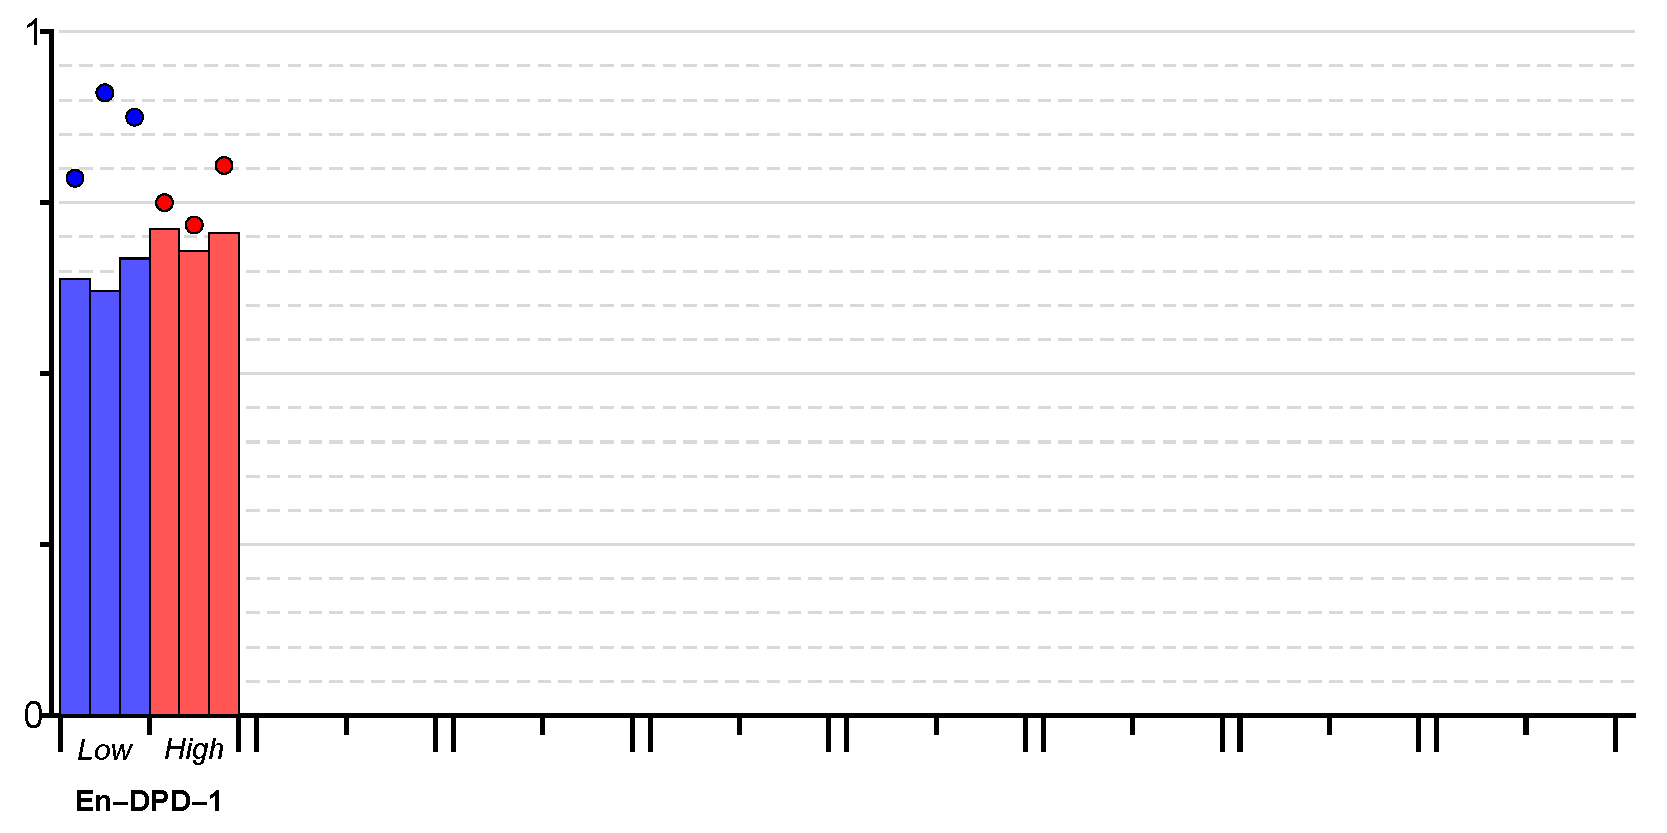
\includegraphics[width=1\textwidth]{./i/col_bar_StateCoop_block_EnDPD_1.pdf}
    \end{center}
\end{card}
\end{frame}

\begin{frame}{Subject-level Cooperation }
\begin{card}
    \begin{center}
    	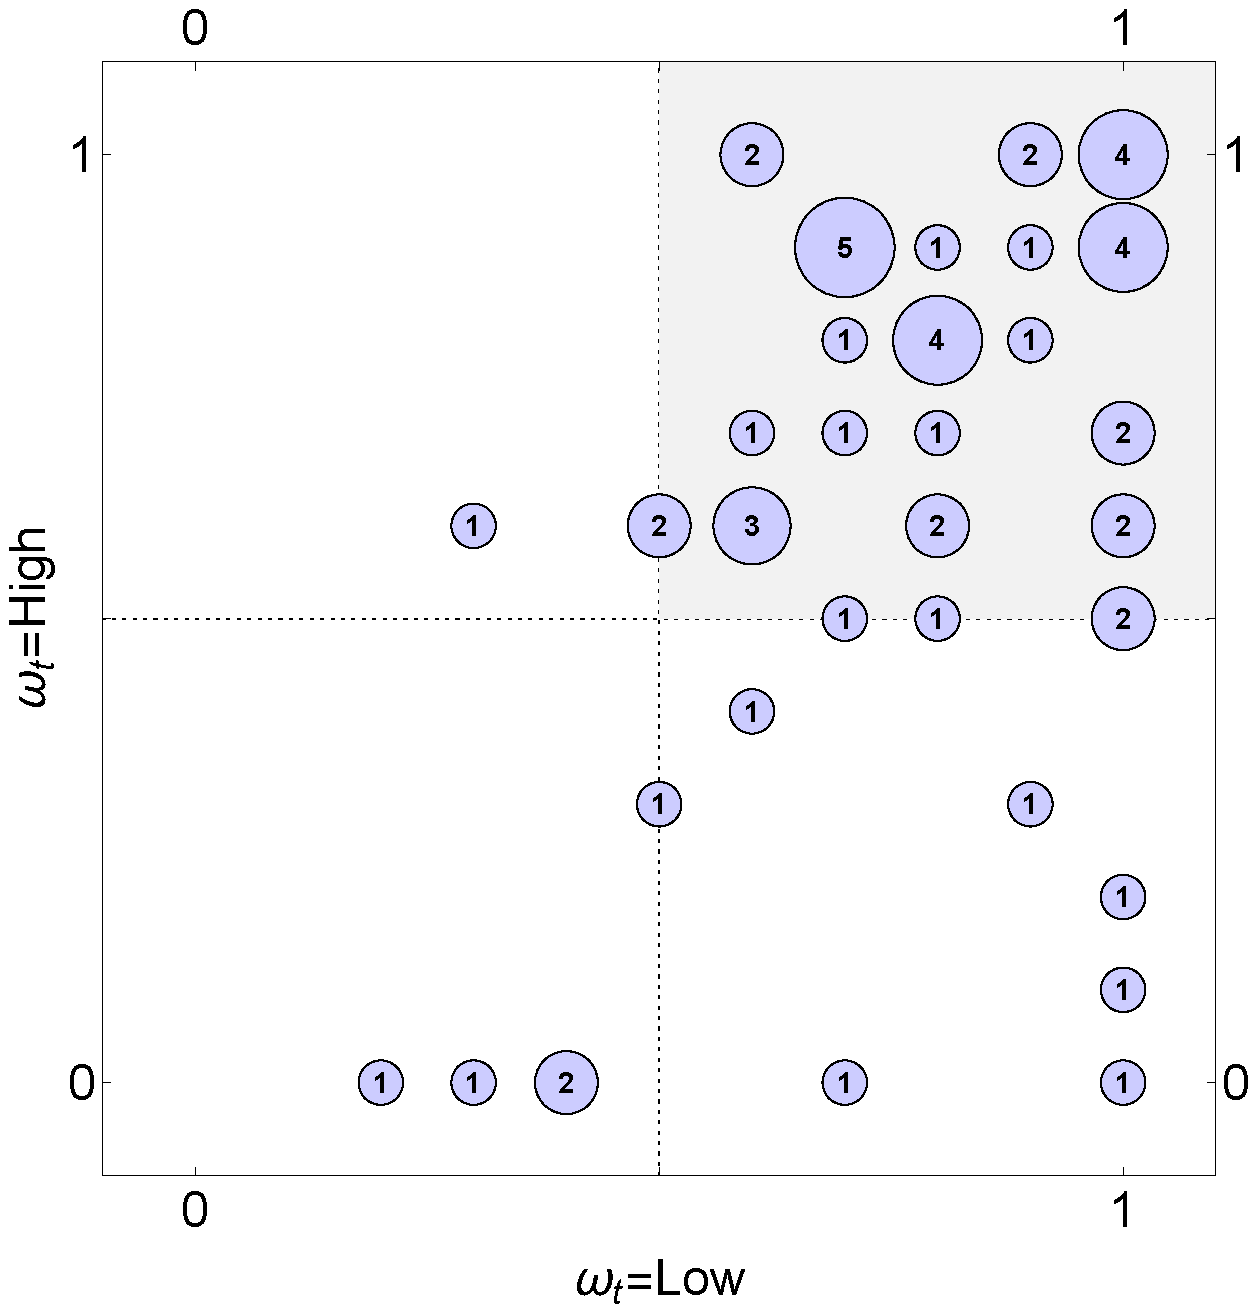
\includegraphics[width=0.6\textwidth]{./i/col_subject_stateCooperation_L5_EnDPD_1.pdf}
    \end{center}
\end{card}
\end{frame}

\begin{frame}{Strategies: SFEM Mixture Model}
\begin{card}
Popular pure strategy Markov:
\begin{itemize}
\item C-C 14.9\%
\item C-D 7.4\% (the MPE)
\item D-D/D-C 7.1\%
\end{itemize}
\end{card}
\begin{card}
 Popular history-dependent strategies
\begin{itemize}
\item Grim trigger 19.2\%
\item C-Alternate-in-high, grim trigger 20.7\%
\end{itemize}
\end{card}
\end{frame}

\begin{frame}
\begin{card}[Result 1]
Not all dynamic games lead to the selection of MPE outcomes;
still observe a lot of conditional cooperation
\end{card}
\end{frame}

\begin{frame}
\begin{card}
\begin{center}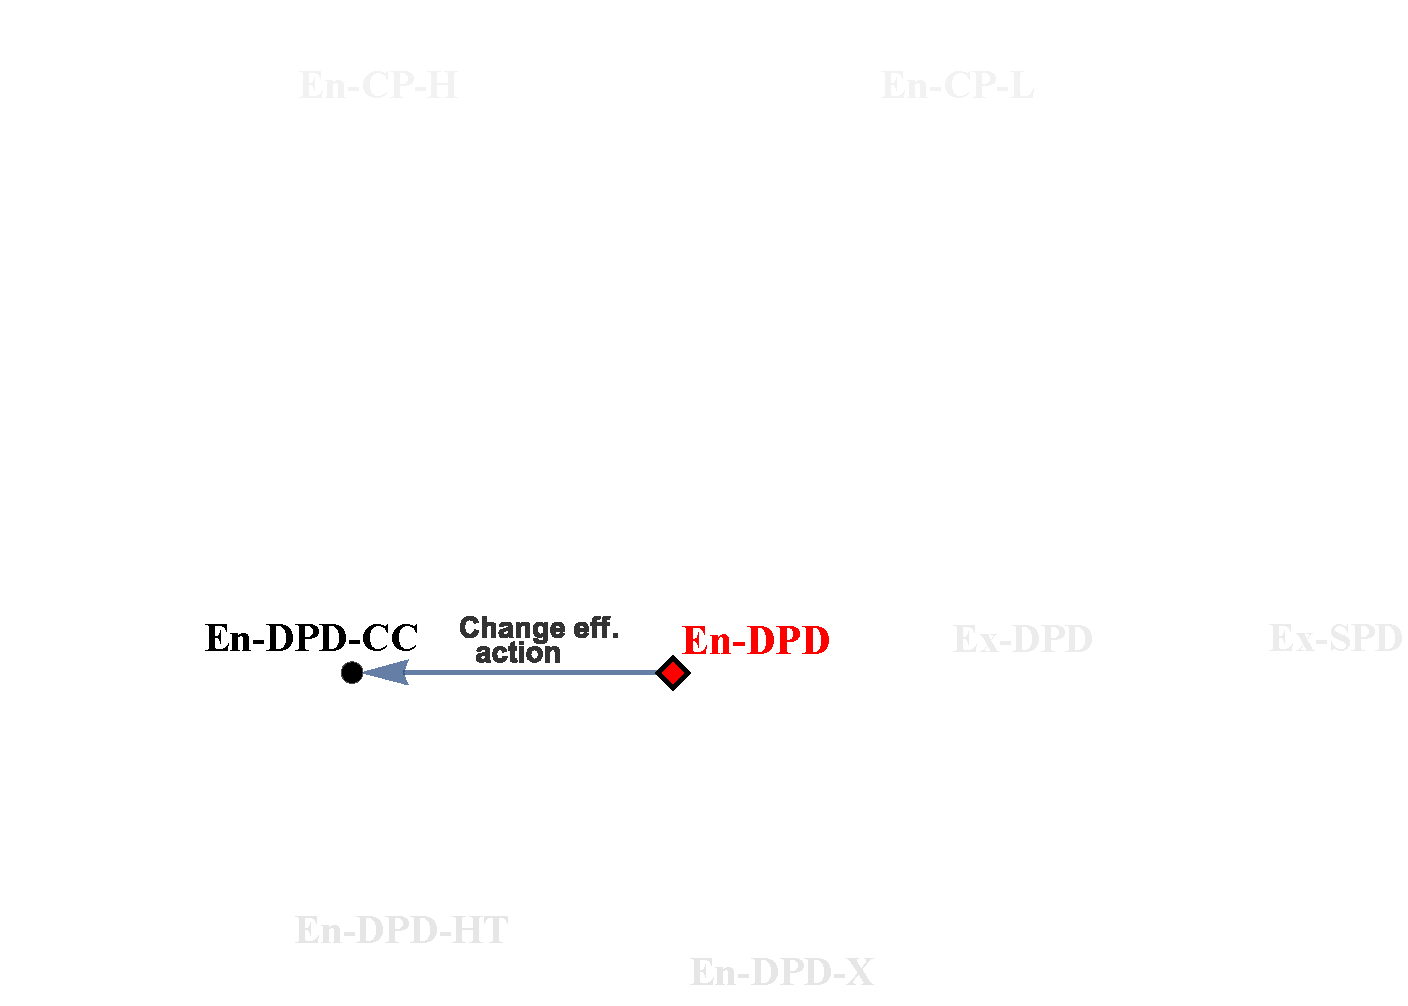
\includegraphics[height=0.7\textwidth]{./i/FlowChart2.pdf}
\end{center}
\end{card}
\end{frame}


\begin{frame}{En-DPD-CC $\rightarrow$ En-DPD}
\begin{card}[Manipulation 1]
Alter the efficient frontier in high
   \begin{itemize}
    \item Increase temptation to defect in high
    \item Make efficient action harder: C/D alternation in high
    \end{itemize}
\end{card}
\end{frame}

\begin{frame}{Endog-Dynamic-PD (Pivot)}
\begin{center}
\begin{table}
\centering{}\subfloat{\centering{}{\small{}}%
\begin{tabular}{ccP{0.1\textwidth}|P{0.1\textwidth}}
\multicolumn{4}{c}{\textcolor{red}{$\omega$=Low}}\\ 

 &  & \multicolumn{2}{c}{2}\\ 
 &  & \multicolumn{1}{P{0.1\textwidth}}{\textbf{C}} & D\\ 
\cline{3-4}
\multirow{2}{*}{1} & \multicolumn{1}{c|}{\textbf{C}} & \textcolor{blue}{100} & \multicolumn{1}{P{0.1\textwidth}|}{\textcolor{red}{30}}\\ 
\cline{3-4}
 & \multicolumn{1}{c|}{D} & \textcolor{red}{125} & \multicolumn{1}{P{0.1\textwidth}|}{\textcolor{red}{60}}\\ 
\cline{3-4}
\end{tabular}}\subfloat{\centering{}{\small{}}%
\begin{tabular}{ccP{0.1\textwidth}|P{0.1\textwidth}}
\multicolumn{4}{c}{\textcolor{blue}{$\omega$=High}}\\ 

 &  & \multicolumn{2}{c}{2}\\ 
 &  & \multicolumn{1}{P{0.1\textwidth}}{C} & \textbf{D}\\ 
\cline{3-4}
\multirow{2}{*}{1} & \multicolumn{1}{c|}{C} & \textcolor{blue}{200} & \multicolumn{1}{P{0.1\textwidth}|}{\textcolor{blue}{130}}\\ 
\cline{3-4}
 & \multicolumn{1}{c|}{\textbf{D}} & \textcolor{blue}{\only<1>{250}\only<2>{280}} & \multicolumn{1}{P{0.1\textwidth}|}{\textbf{\textcolor{red}{190}}}\\ 
\cline{3-4}
\end{tabular}}
\end{table}
\end{center}


\textrm{
\[
\psi\left(\mbox{\ensuremath{\omega}},a\right)=\begin{cases}
\mbox{High} & \mbox{if }a=\left(C,C\right),\mbox{\ensuremath{\omega}=Low}\\
\mbox{Low} & \mbox{if }a=\left(D,D\right),\mbox{\ensuremath{\omega}=High}\\
\omega & \mbox{otherwise}
\end{cases}
\]
\pause}


Unique MPE still: $\alpha_{i}^{\star}(\omega)=\begin{cases}
\mbox{C} & \mbox{if \ensuremath{\omega}=Low}\\
\mbox{D} & \mbox{if \ensuremath{\omega}=High}
\end{cases}$

\end{frame}

\begin{frame}{Dynamic PD Game-1}
\begin{card}
    \begin{center}
    	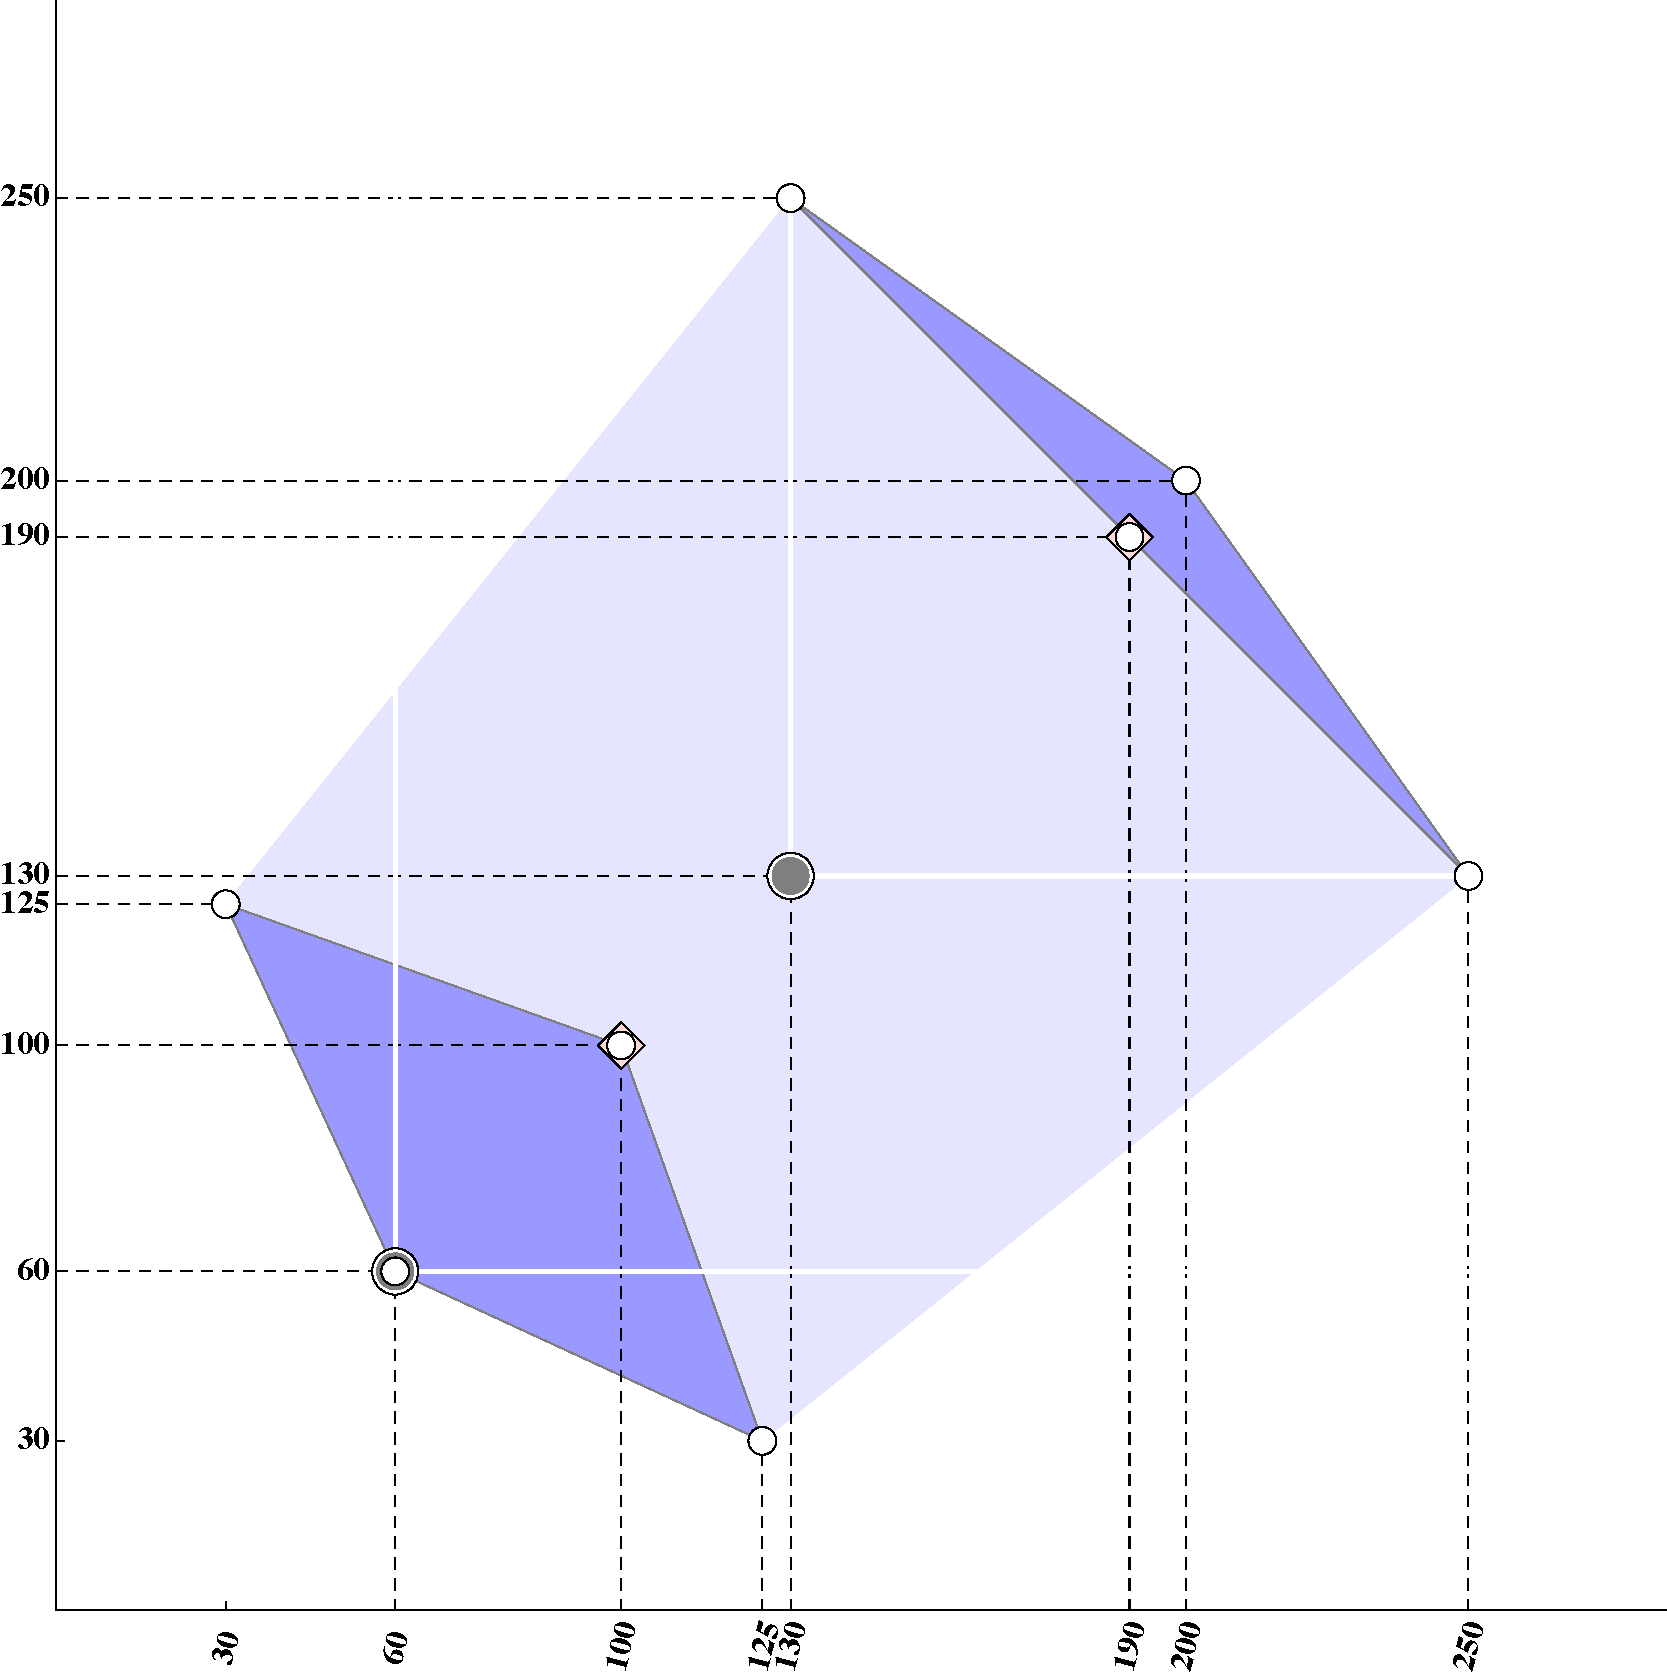
\includegraphics[width=0.6\textwidth]{./i/col_GamePayoffs1.pdf}
    \end{center}
\end{card}
\end{frame}
\begin{frame}{Dynamic PD Game-2}
\begin{card}
    \begin{center}
    	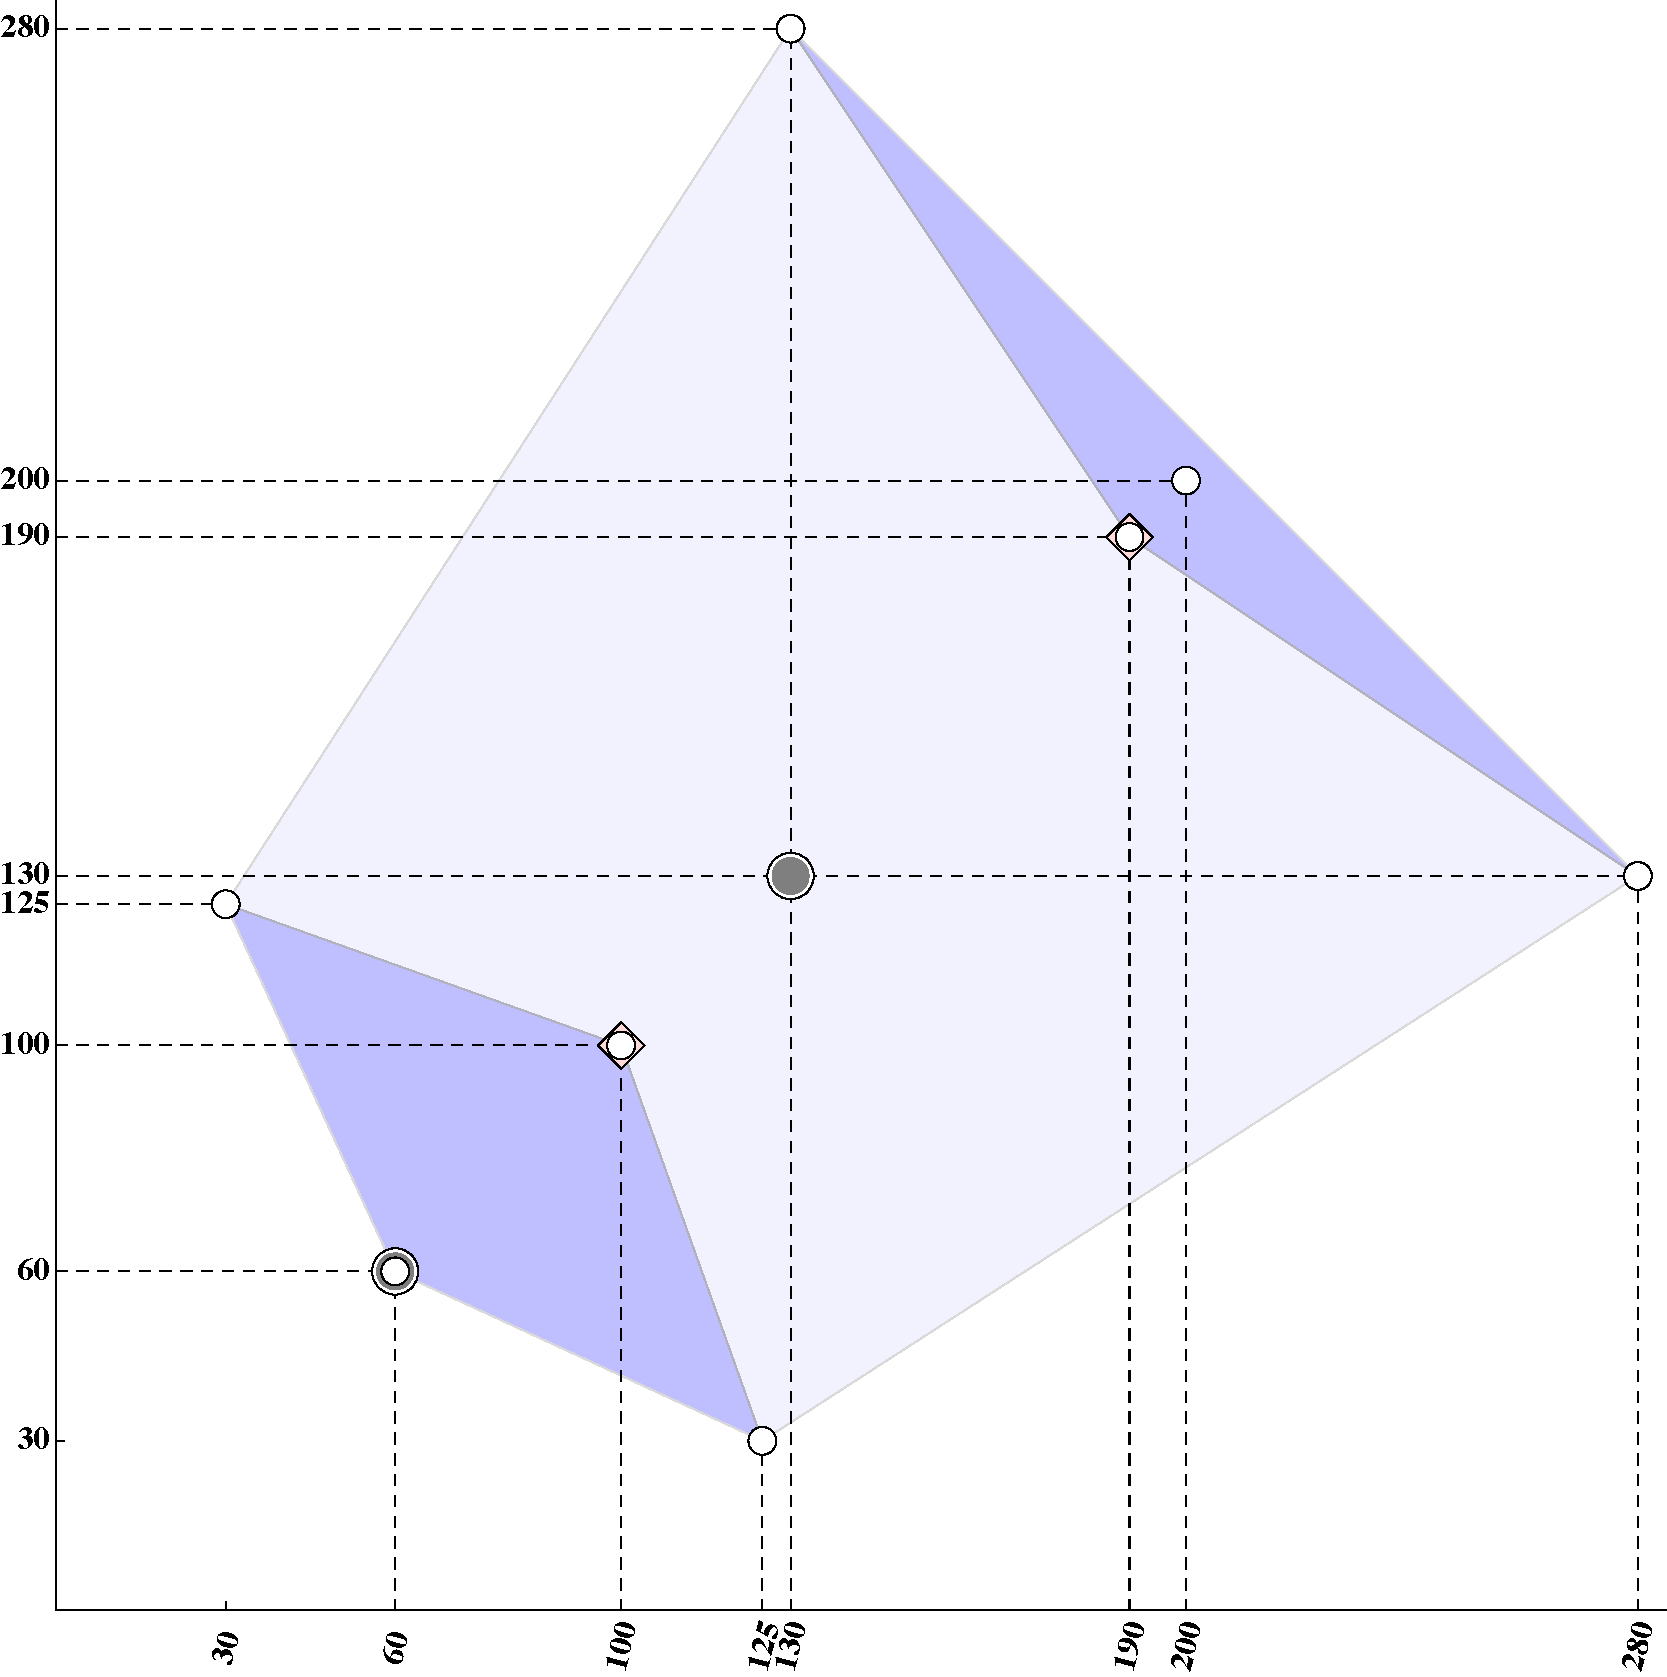
\includegraphics[width=0.6\textwidth]{./i/col_GamePayoffs2.pdf}
    \end{center}
\end{card}
\end{frame}

\begin{frame}{Results: Cooperation by State}
\begin{card}
\begin{center}
	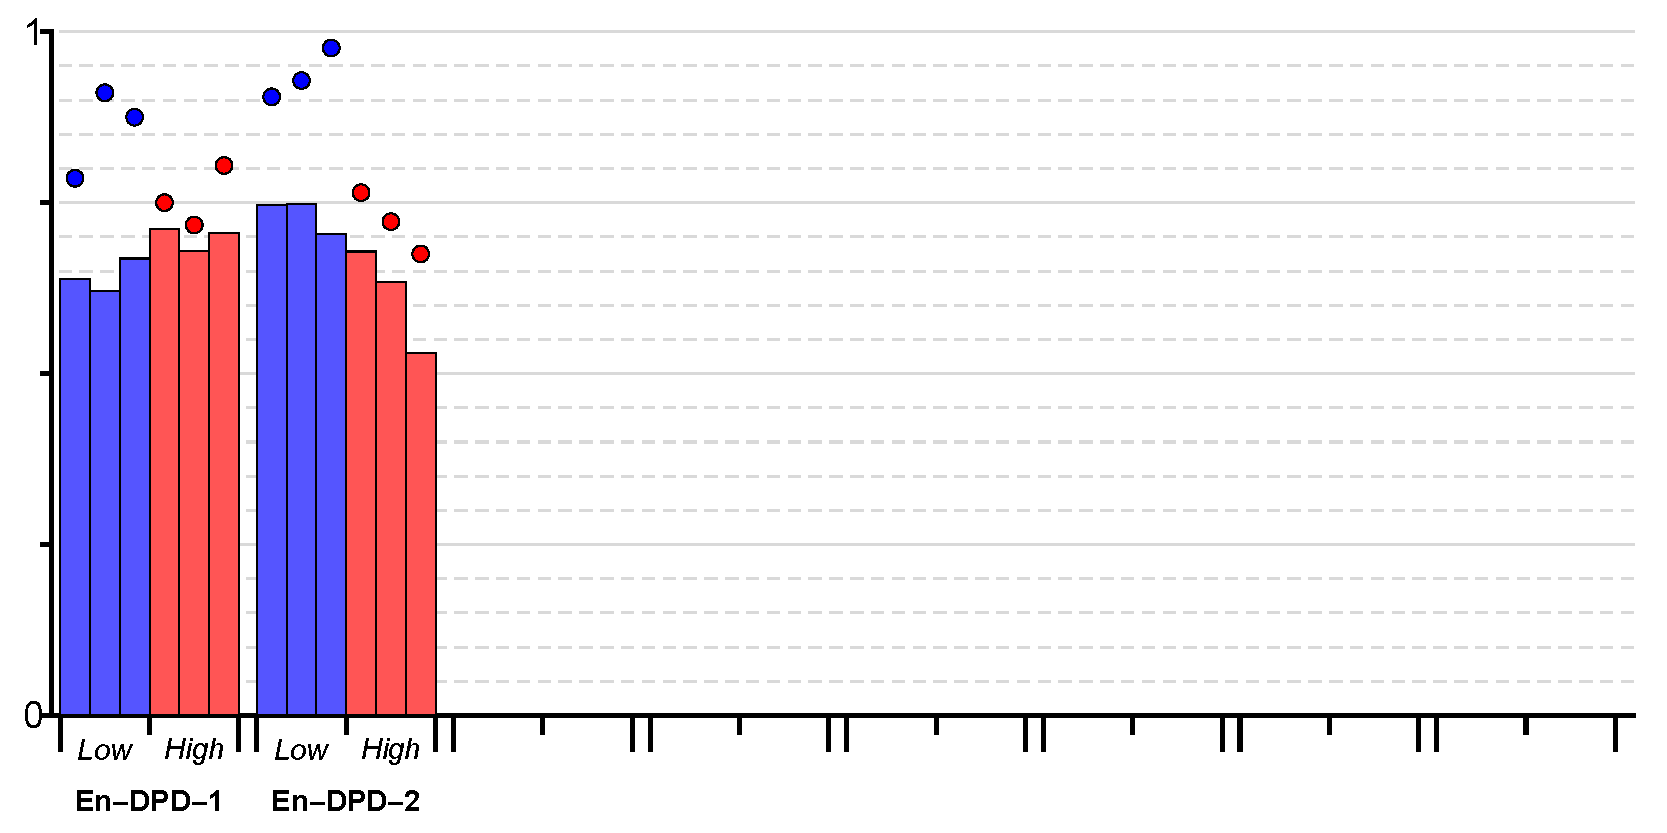
\includegraphics[width=1.0\textwidth]{./i/col_bar_StateCoop_block_EnDPD_2.pdf}
\end{center}

\end{card}
\end{frame}

\begin{frame}{Subject Cooperation:En-DPD }
\begin{card}
\begin{center}
	\includegraphics<2>[width=0.6\textwidth]{./i/col_subject_stateCooperation_L5_EnDPD_2.pdf}
\end{center}
\end{card}
\end{frame}

\begin{frame}{Strategies}
\begin{card}
Popular pure strategy Markov:

\begin{itemize}
\item C-C: $14.9\%\rightarrow7.9\%$
\item C-D: $7.1\%\rightarrow23.5\%$
\item D-D: $7.4\%\rightarrow4.7\%$
\end{itemize}
\end{card}

\begin{card} Popular history-dependent strategies
\begin{itemize}
\item Grim trigger $19.2\%\rightarrow13.8\%$
\item C-Alternate-in-high, grim trigger $20.7\%\rightarrow0\%$
\item D-Alternate-in-high, grim trigger $1.5\%\rightarrow16.2\%$
\item C-Alternate-in-high, MPE-trigger $5.8\%\rightarrow28.7\%$
\end{itemize}
\end{card}
\end{frame}


\begin{frame}
\begin{card}[Result 2]
Conditional cooperation here moves to support the efficient
outcome, though C/D alternation in High was common even when joint
cooperation was efficient
\end{card}
\end{frame}

\begin{frame}
\begin{card}
\begin{center}
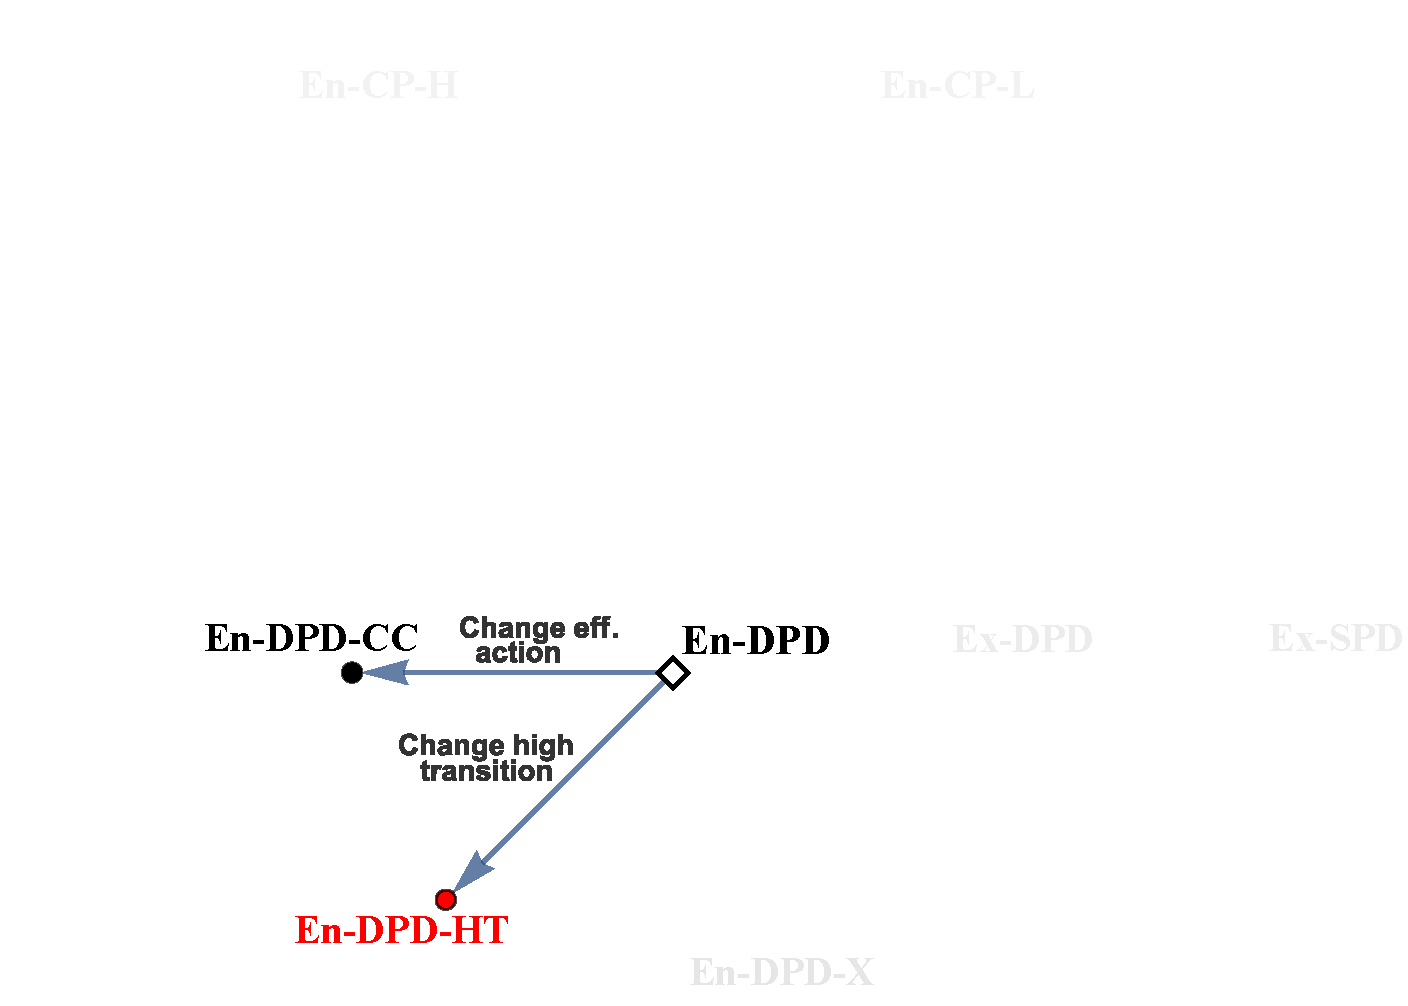
\includegraphics[height=0.7\textwidth]{./i/FlowChart3.pdf}
\end{center}
\end{card}
\end{frame}


\begin{frame}{En-DPD $\rightarrow$ En-DPD-HT}
\begin{card}
\begin{itemize}
\item From En-DPD (the pivot) only (D,D) in high causes Low next round
\item Subjects can unilaterally impose the high state once there
\end{itemize}
\end{card}
\begin{card}[Manipulation 2]
 Change transition rule in high state
    \begin{itemize}
    \item Require joint cooperation to stay in High
    \item (D,D), (C,D) and (D,C) in High lead to Low next round
    \end{itemize}
\end{card}
\end{frame}

\begin{frame}{Endog-Dynamic-PD$\rightarrow$}
\begin{center}
\begin{table}
\centering{}\subfloat{\centering{}{\small{}}%
\begin{tabular}{ccP{0.1\textwidth}|P{0.1\textwidth}}
\multicolumn{4}{c}{\textcolor{red}{$\omega$=Low}}\\ 

 &  & \multicolumn{2}{c}{2}\\ 
 &  & \multicolumn{1}{P{0.1\textwidth}}{\textbf{C}} & D\\ 
\cline{3-4}
\multirow{2}{*}{1} & \multicolumn{1}{c|}{\textbf{C}} & \textcolor{blue}{100} & \multicolumn{1}{P{0.1\textwidth}|}{\textcolor{red}{30}}\\ 
\cline{3-4}
 & \multicolumn{1}{c|}{D} & \textcolor{red}{125} & \multicolumn{1}{P{0.1\textwidth}|}{\textcolor{red}{60}}\\ 
\cline{3-4}
\end{tabular}}\subfloat{\centering{}{\small{}}%
\begin{tabular}{ccP{0.1\textwidth}|P{0.1\textwidth}}
\multicolumn{4}{c}{\textcolor{blue}{$\omega$=High}}\\ 

 &  & \multicolumn{2}{c}{2}\\ 
 &  & \multicolumn{1}{P{0.1\textwidth}}{C} & \textbf{D}\\ 
\cline{3-4}
\multirow{2}{*}{1} & \multicolumn{1}{c|}{C} & \textcolor{blue}{200} & \multicolumn{1}{P{0.1\textwidth}|}{\textcolor{blue}{130}}\\ 
\cline{3-4}
 & \multicolumn{1}{c|}{\textbf{D}} & \textcolor{blue}{280} & \multicolumn{1}{P{0.1\textwidth}|}{\textcolor{red}{190}}\\ 
\cline{3-4}
\end{tabular}}
\end{table}

\par\end{center}

\begin{center}
\[
\psi\left(\mbox{\ensuremath{\omega}},a\right)=\begin{cases}
\mbox{High} & \mbox{if }a=\left(C,C\right),\mbox{\ensuremath{\omega}=Low}\\
\mbox{Low} & \mbox{if }a=\left(D,D\right),\mbox{\ensuremath{\omega}=High}\\
\omega & \mbox{otherwise}
\end{cases}
\]

\par\end{center}

$C-D$ unique MPE.

\end{frame}

\begin{frame}{Endog-Dynamic-PD-2$\rightarrow$Endog-Dynamic-PD-HT}

\begin{center}
\begin{table}
\centering{}\subfloat{\centering{}{\small{}}%
\begin{tabular}{ccP{0.1\textwidth}|P{0.1\textwidth}}
\multicolumn{4}{c}{\textcolor{red}{$\omega$=Low}}\\ 

 &  & \multicolumn{2}{c}{2}\\ 
 &  & \multicolumn{1}{P{0.1\textwidth}}{\textbf{C}} & D\\ 
\cline{3-4}
\multirow{2}{*}{1} & \multicolumn{1}{c|}{\textbf{C}} & \textcolor{blue}{100} & \multicolumn{1}{P{0.1\textwidth}|}{\textcolor{red}{30}}\\ 
\cline{3-4}
 & \multicolumn{1}{c|}{D} & \textcolor{red}{125} & \multicolumn{1}{P{0.1\textwidth}|}{\textcolor{red}{60}}\\ 
\cline{3-4}
\end{tabular}}\subfloat{\centering{}{\small{}}%
\begin{tabular}{ccP{0.1\textwidth}|P{0.1\textwidth}}
\multicolumn{4}{c}{\textcolor{blue}{$\omega$=High}}\\ 

 &  & \multicolumn{2}{c}{2}\\ 
 &  & \multicolumn{1}{P{0.1\textwidth}}{C} & \textbf{D}\\ 
\cline{3-4}
\multirow{2}{*}{1} & \multicolumn{1}{c|}{C} & \textcolor{blue}{200} & \multicolumn{1}{P{0.1\textwidth}|}{\textcolor{red}{130}}\\ 
\cline{3-4}
 & \multicolumn{1}{c|}{\textbf{D}} & \textcolor{red}{280} & \multicolumn{1}{P{0.1\textwidth}|}{\textcolor{red}{190}}\\ 
\cline{3-4}
\end{tabular}}
\end{table}

\par\end{center}

\begin{center}
\[
\psi\left(\mbox{\ensuremath{\omega}},a\right)=\begin{cases}
\mbox{High} & \mbox{if }a=\left(C,C\right)\\
\mbox{Low} & \mbox{otherwise.}
\end{cases}
\]

\par\end{center}
\begin{itemize}
\item $C-D$ still MPE, but $D-D$ now also
\item $D-C$ is an MPE, but starting state is \emph{Low}
\end{itemize}
\end{frame}
\begin{frame}{Results: Cooperation by State}
\begin{card}
    \begin{center}
    	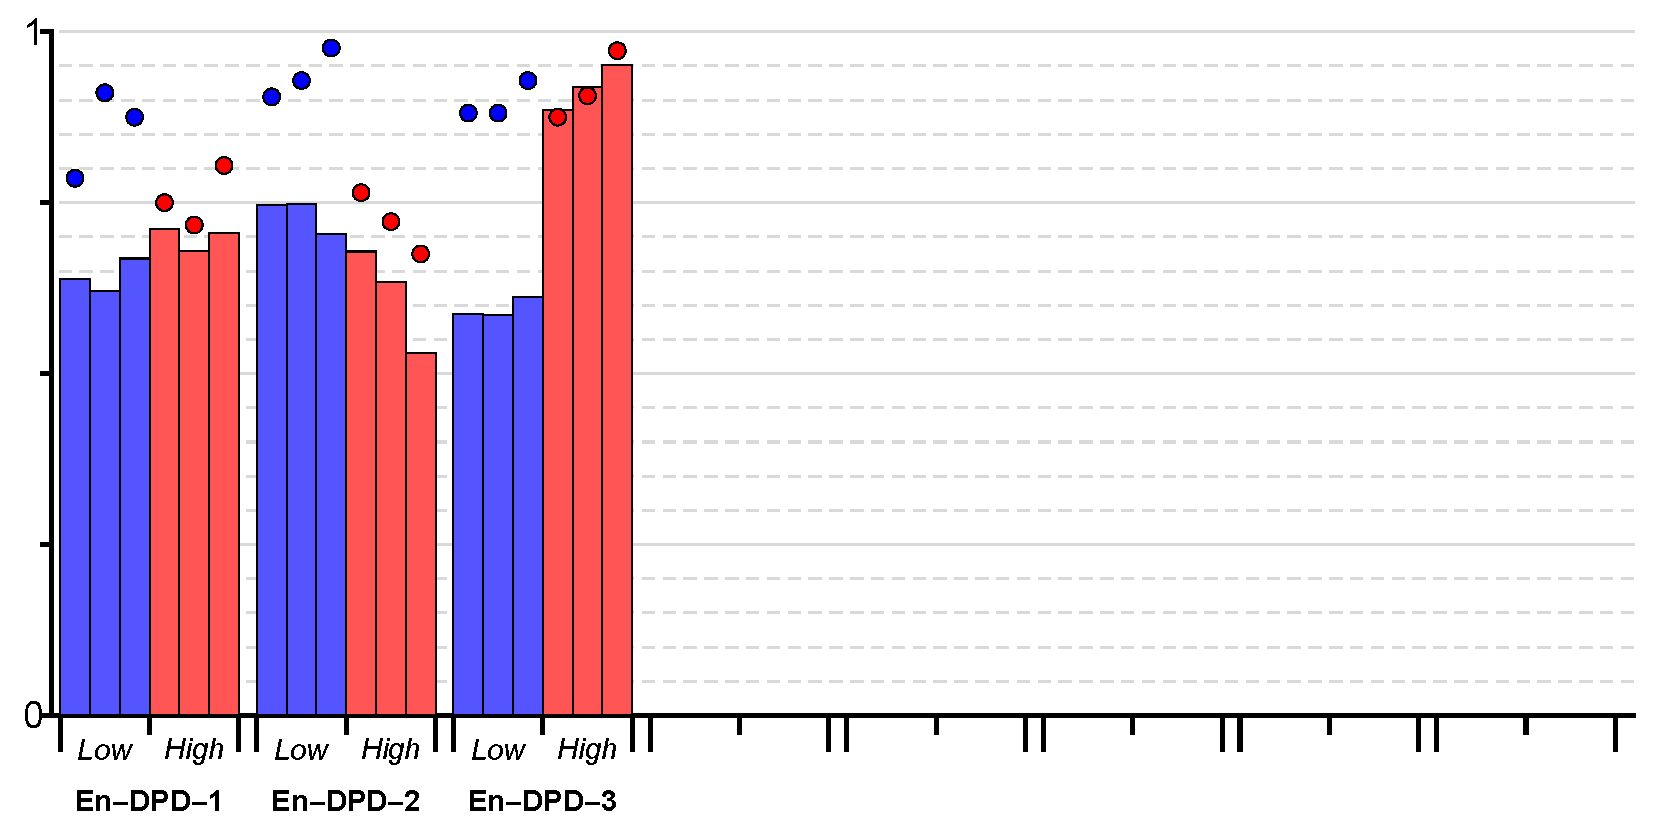
\includegraphics[width=1.0\textwidth]{./i/col_bar_StateCoop_block_EnDPD_H.pdf}
    \end{center}
\end{card}
\end{frame}

\begin{frame}{Subject Cooperation:En-DPD-HT }
\begin{card}
    \begin{center}
    	\includegraphics<2>[width=0.6\textwidth]{./i/col_subject_stateCooperation_L5_EnDPD_H.pdf}
    \end{center}
\end{card}
\end{frame}


\begin{frame}{Strategies (En-DPD$\rightarrow$En-DPD-HT)}

    \begin{card}
     Popular pure strategy Markov:
    \begin{itemize}
    \item C-C: $7.9\%\rightarrow24.5\%$
    \item C-D: $23.5\%\rightarrow2.0\%$
    \item D-D: $4.7\%\rightarrow2.4\%$
    \end{itemize}
    \end{card}
    \begin{card}
    Popular history-dependent strategies
    
    \begin{itemize}
    \item Grim trigger $13.8\%\rightarrow34.0\%$
    \end{itemize}
    \end{card}
\end{frame}

\begin{frame}

\begin{card}[Result 3:]
Reducing the IR payoff increases cooperation, punishments
used are harsher
\end{card}
\end{frame}

\begin{frame}
\begin{card}
\begin{center}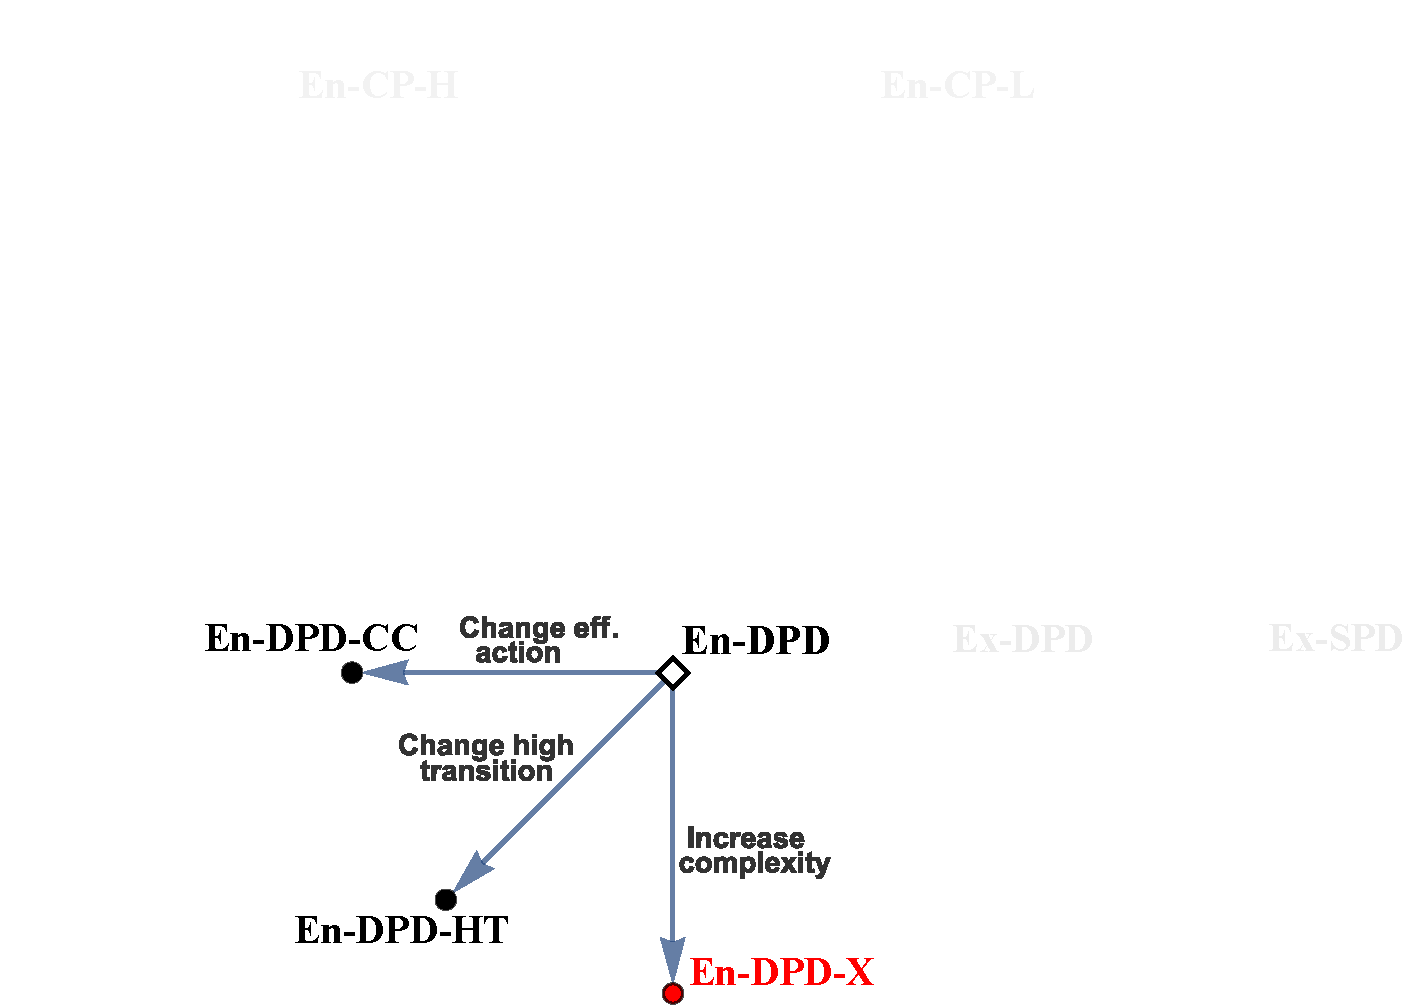
\includegraphics[height=0.7\textwidth]{./i/FlowChart4.pdf}
\end{center}
\end{card}
\end{frame}


\begin{frame}{En-DPD $\rightarrow$ En-DPD-X}

\begin{card}
Computational complexity literature identifies complexity as one reason
to select MPE (in particular the number of payoff relevant states)
\end{card}
\pause

\begin{card}[Manipulation 3:] 
Make the game more complex
    \begin{itemize}
    \item Same game as En-DPD with added exogenous shocks each round
    \item Draw a number $x$ uniformly over $X=\left\{ -5,-4,\ldots,4,5\right\} $
    \item 2 states $\rightarrow$ 22 states.
    \end{itemize}
\end{card}
\end{frame}

\begin{frame}{Complex Endog-Dynamic-PD}
\begin{center}
\begin{table}
\centering{}\subfloat{\centering{}{\small{}}%
\begin{tabular}{ccP{0.1\textwidth}|P{0.1\textwidth}}
\multicolumn{4}{c}{\textcolor{red}{$\omega$=Low}}\\ 

 &  & \multicolumn{2}{c}{2}\\ 
 &  & \multicolumn{1}{P{0.1\textwidth}}{\textbf{C}} & D\\ 
\cline{3-4}
\multirow{2}{*}{1} & \multicolumn{1}{c|}{\textbf{C}} & \textcolor{blue}{100+x} & \multicolumn{1}{P{0.1\textwidth}|}{\textcolor{red}{30+x}}\\ 
\cline{3-4}
 & \multicolumn{1}{c|}{D} & \textcolor{red}{125-x} & \multicolumn{1}{P{0.1\textwidth}|}{\textcolor{red}{60-x}}\\ 
\cline{3-4}
\end{tabular}}\subfloat{\centering{}{\small{}}%
\begin{tabular}{ccP{0.12\textwidth}|P{0.12\textwidth}}
\multicolumn{4}{c}{\textcolor{blue}{$\omega$=High}}\\ 
 &  & \multicolumn{1}{P{0.12\textwidth}}{} & \\ 
 &  & \multicolumn{2}{c}{2}\\ 
 &  & \multicolumn{1}{P{0.12\textwidth}}{C} & \textbf{D}\\ 
\cline{3-4}
\multirow{2}{*}{1} & \multicolumn{1}{c|}{C} & \textcolor{blue}{200+2x} & \multicolumn{1}{P{0.12\textwidth}|}{\textcolor{blue}{130+2x}}\\ 
\cline{3-4}
 & \multicolumn{1}{c|}{\textbf{D}} & \textcolor{blue}{280-2x} & \multicolumn{1}{P{0.12\textwidth}|}{\textbf{\textcolor{red}{190-2x}}}\\ 
\cline{3-4}
\end{tabular}}
\end{table}
\end{center}

\[
\psi\left(\mbox{\ensuremath{\omega}},a\right)=\begin{cases}
\left(\mbox{High},y\right) & \mbox{if }a=\left(C,C\right),\omega=\left(\mbox{Low},x\right)\\
\left(\mbox{Low},y\right) & \mbox{if }a=\left(D,D\right),\omega=\left(\mbox{High},x\right)\\
\left(\omega_{1},y\right) & \mbox{otherwise}
\end{cases}
\]
\begin{itemize}
\item $y\perp x$, uniformly distributed on $\left\{ -5,-4,\ldots,4,5\right\} $
\item $C-D$ in \emph{Low/High} and ignoring $x$ an MPE (not unique though)
\end{itemize}
\end{frame}


\begin{frame}{Results: Cooperation by State}
\begin{card}
\begin{center}
	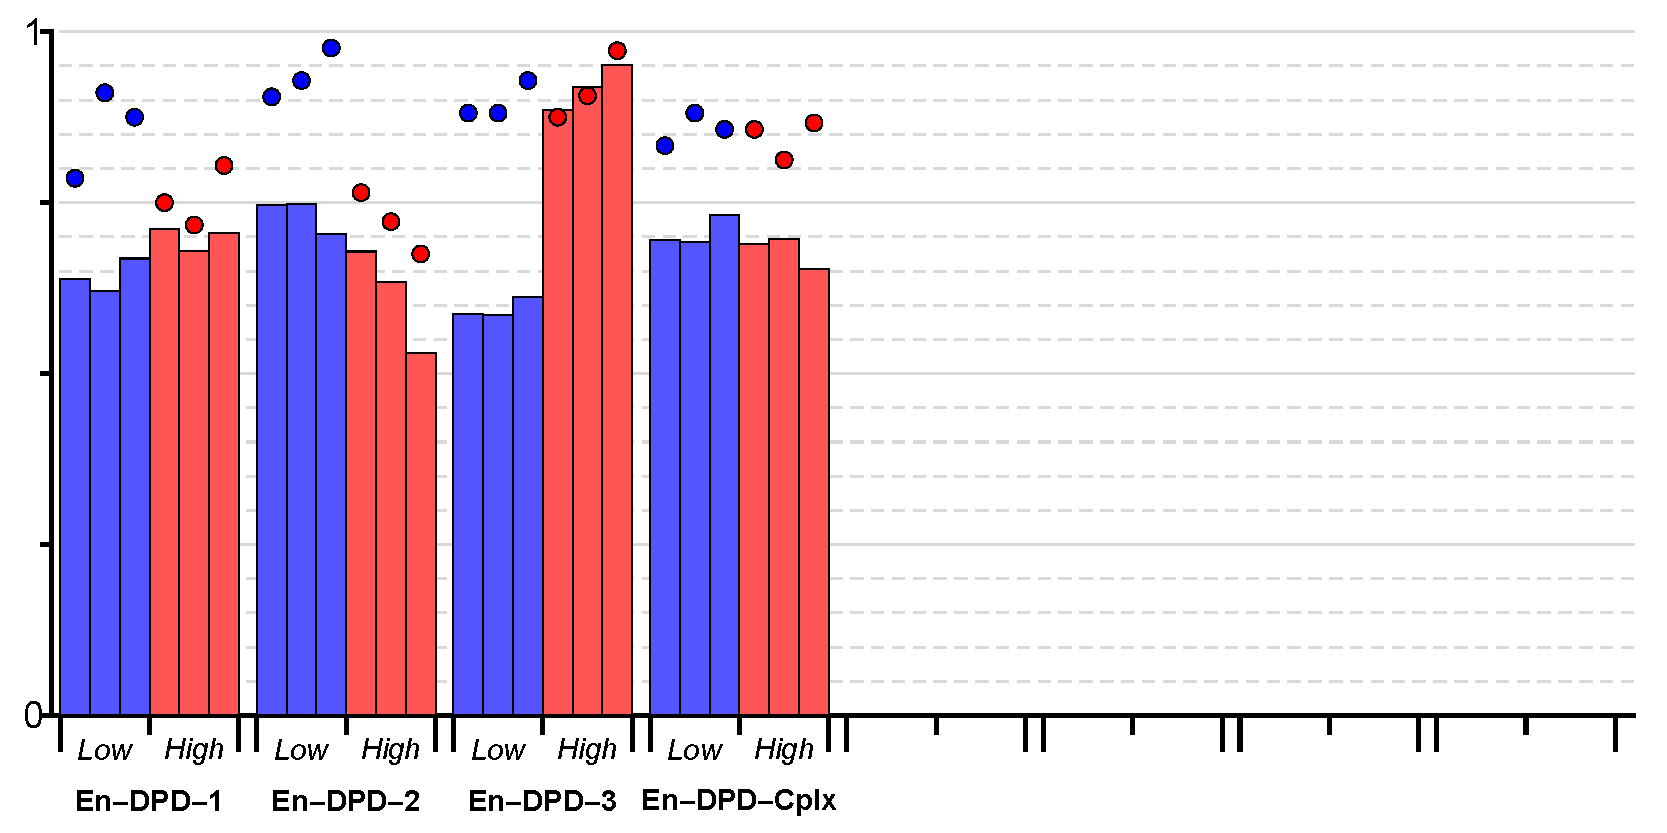
\includegraphics[width=1.0\textwidth]{./i/col_bar_StateCoop_block_EnDPD_C.pdf}
\end{center}
\end{card}
\end{frame}

\begin{frame}{Strategies (En-DPD$\rightarrow$En-DPD-X)}
\begin{card}
 Markov strategies:
\begin{itemize}
\item C-C: $7.9\%\rightarrow31.4\%$
\item \textbf{C-D:} $23.5\%\rightarrow19.1\%$
\item D-D\textbf{:} $4.7\%\rightarrow2.7\%$
\end{itemize}
\end{card}
\begin{card}
Popular history-dependent strategies
\begin{itemize}
\item MPE-trigger $7.8\%\rightarrow19.0\%$
\item C-Alternate, MPE-trigger $23.4\%\rightarrow14.2\%$
\end{itemize}
\end{card}
\end{frame}

\begin{frame}
\begin{card}[Result 4]
Small changes to the games payoffs lead to small deviations
in behavior even with much increased complexity. Increased complexity
does not lead to increased selection of MPE.
\end{card}
\end{frame}


\begin{frame}{Dynamic PD game summary}

\begin{card}
Across a series of manipulations to a similar Dynamic PD game we find
effects over:

\begin{itemize}
\item where conditional cooperation is targeted
\item the types of punishments that support it
\end{itemize}
But little differences in rate of MPE selection. Turn instead to changing the nature of the dynamics
\end{card}
\end{frame}

\begin{frame}
\begin{card}
\begin{center}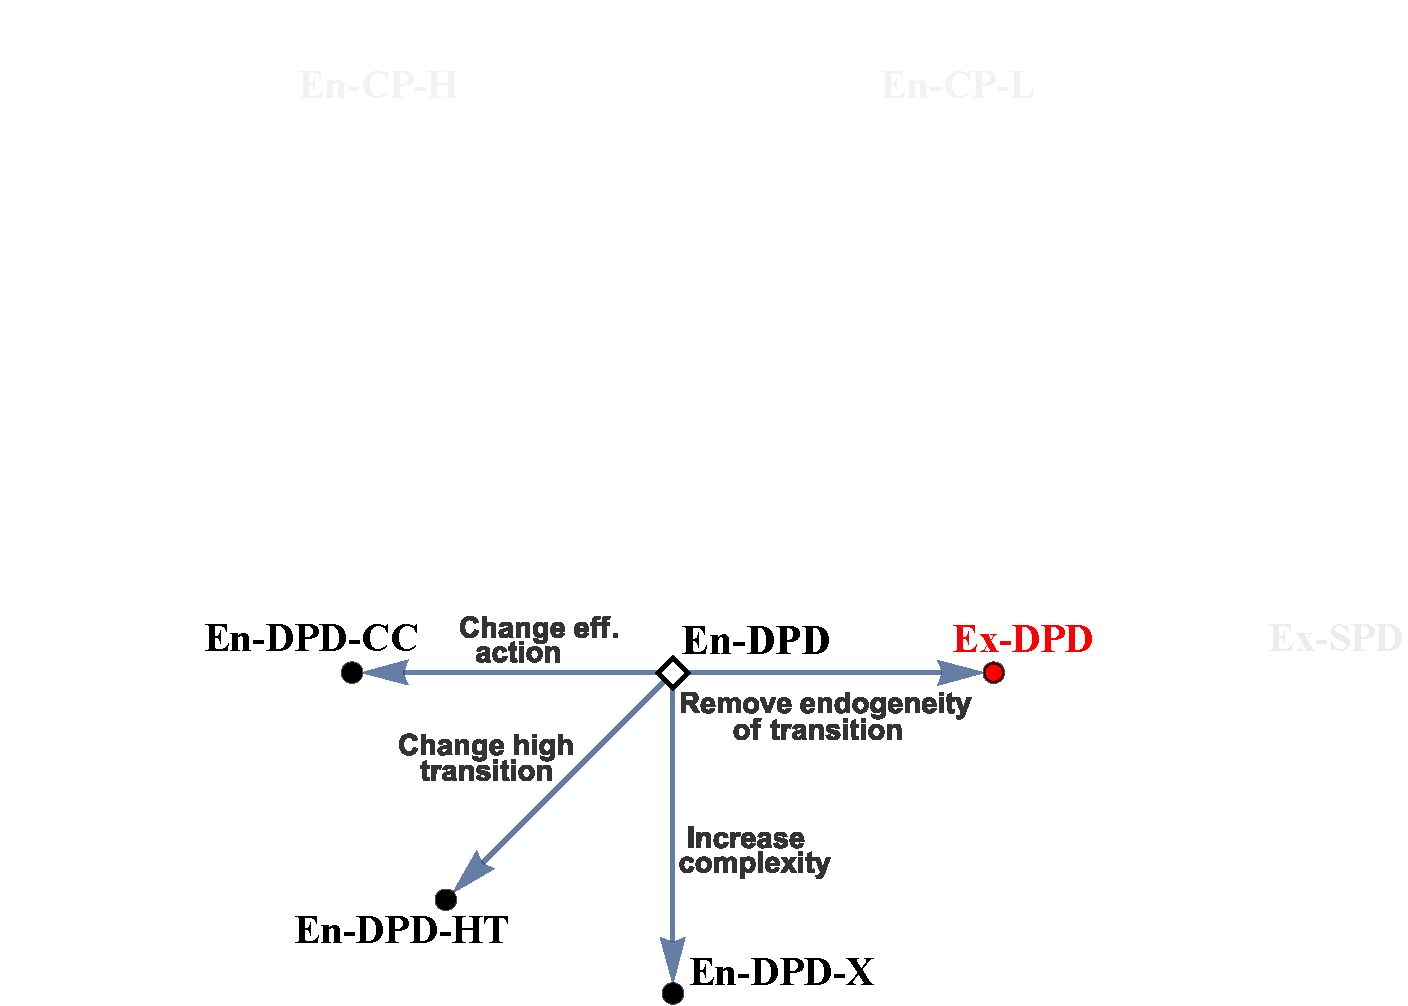
\includegraphics[height=0.7\textwidth]{./i/FlowChart5.pdf}
\end{center}
\end{card}
\end{frame}

\begin{frame}{En-DPD-2 $\rightarrow$ Ex-DPD-2}
\begin{card}
 In the En-DPD games the transitions are endogenous, so there is a
dynamic externality (actions affect the state, which affects the other player's payoff)

What are the effects of removing the dynamic externality?
\end{card}
\pause

    \begin{card}[Manipulation 4:] 
    Eliminate the dynamic externality
        \begin{itemize}
        \item Exogenous random transition between states
        \item Choose probabilities to match observed state frequency in En-DPD
        \end{itemize}
    \end{card}
\end{frame}

\begin{frame}{Endog-Dynamic-PD}

\begin{center}
\begin{table}
\centering{}\subfloat{\centering{}{\small{}}%
\begin{tabular}{ccP{0.1\textwidth}|P{0.1\textwidth}}
\multicolumn{4}{c}{\textcolor{red}{$\omega$=Low}}\\ 

 &  & \multicolumn{2}{c}{2}\\ 
 &  & \multicolumn{1}{P{0.1\textwidth}}{\textbf{C}} & D\\ 
\cline{3-4}
\multirow{2}{*}{1} & \multicolumn{1}{c|}{\textbf{C}} & \textcolor{blue}{100} & \multicolumn{1}{P{0.1\textwidth}|}{\textcolor{red}{30}}\\ 
\cline{3-4}
 & \multicolumn{1}{c|}{D} & \textcolor{red}{125} & \multicolumn{1}{P{0.1\textwidth}|}{\textcolor{red}{60}}\\ 
\cline{3-4}
\end{tabular}}\subfloat{\centering{}{\small{}}%
\begin{tabular}{ccP{0.1\textwidth}|P{0.1\textwidth}}
\multicolumn{4}{c}{\textcolor{blue}{$\omega$=High}}\\ 

 &  & \multicolumn{2}{c}{2}\\ 
 &  & \multicolumn{1}{P{0.1\textwidth}}{C} & \textbf{D}\\ 
\cline{3-4}
\multirow{2}{*}{1} & \multicolumn{1}{c|}{C} & \textcolor{blue}{200} & \multicolumn{1}{P{0.1\textwidth}|}{\textcolor{blue}{130}}\\ 
\cline{3-4}
 & \multicolumn{1}{c|}{\textbf{D}} & \textcolor{blue}{280} & \multicolumn{1}{P{0.1\textwidth}|}{\textbf{\textcolor{red}{190}}}\\ 
\cline{3-4}
\end{tabular}}
\end{table}

\par\end{center}


\[
\psi\left(\mbox{\ensuremath{\omega}},a\right)=\begin{cases}
\mbox{High} & \mbox{if }a=\left(C,C\right),\mbox{\ensuremath{\omega}=Low}\\
\mbox{Low} & \mbox{if }a=\left(D,D\right),\mbox{\ensuremath{\omega}=High}\\
\omega & \mbox{otherwise}
\end{cases}
\]

Unique MPE is C-D
\end{frame}

\begin{frame}{Exog-Dynamic-PD}
\begin{table}
\centering{}\subfloat{\centering{}{\small{}}%
\begin{tabular}{ccP{0.1\textwidth}|P{0.1\textwidth}}
\multicolumn{4}{c}{\textcolor{red}{$\omega$=Low}}\\ 

 &  & \multicolumn{2}{c}{2}\\ 
 &  & \multicolumn{1}{P{0.1\textwidth}}{\textbf{C}} & D\\ 
\cline{3-4}
\multirow{2}{*}{1} & \multicolumn{1}{c|}{\textbf{C}} & \textcolor{black}{100} & \multicolumn{1}{P{0.1\textwidth}|}{\textcolor{black}{30}}\\ 
\cline{3-4}
 & \multicolumn{1}{c|}{D} & \textcolor{black}{125} & \multicolumn{1}{P{0.1\textwidth}|}{\textcolor{black}{60}}\\ 
\cline{3-4}
\end{tabular}}\subfloat{\centering{}{\small{}}%
\begin{tabular}{ccP{0.1\textwidth}|P{0.1\textwidth}}
\multicolumn{4}{c}{\textcolor{blue}{$\omega$=High}}\\ 

 &  & \multicolumn{2}{c}{2}\\ 
 &  & \multicolumn{1}{P{0.1\textwidth}}{C} & \textbf{D}\\ 
\cline{3-4}
\multirow{2}{*}{1} & \multicolumn{1}{c|}{C} & \textcolor{black}{200} & \multicolumn{1}{P{0.1\textwidth}|}{\textcolor{black}{130}}\\ 
\cline{3-4}
 & \multicolumn{1}{c|}{\textbf{D}} & \textcolor{black}{280} & \multicolumn{1}{P{0.1\textwidth}|}{\textbf{\textcolor{black}{190}}}\\ 
\cline{3-4}
\end{tabular}}
\end{table}


\textrm{
\[
\psi\left(\mbox{\ensuremath{\omega}},a\right)=\begin{cases}
0.6\cdot\mbox{High}\oplus0.4\cdot\mbox{Low} & \mbox{if \ensuremath{\omega}=Low}\\
0.8\cdot\mbox{High}\oplus0.2\cdot\mbox{Low} & \mbox{if }\mbox{\ensuremath{\omega}=High}
\end{cases}
\]
}

Unique MPE now $D-D$, but efficient SPE still possible!

\end{frame}

\begin{frame}{Results: Cooperation by State}
\begin{card}
\begin{center}
	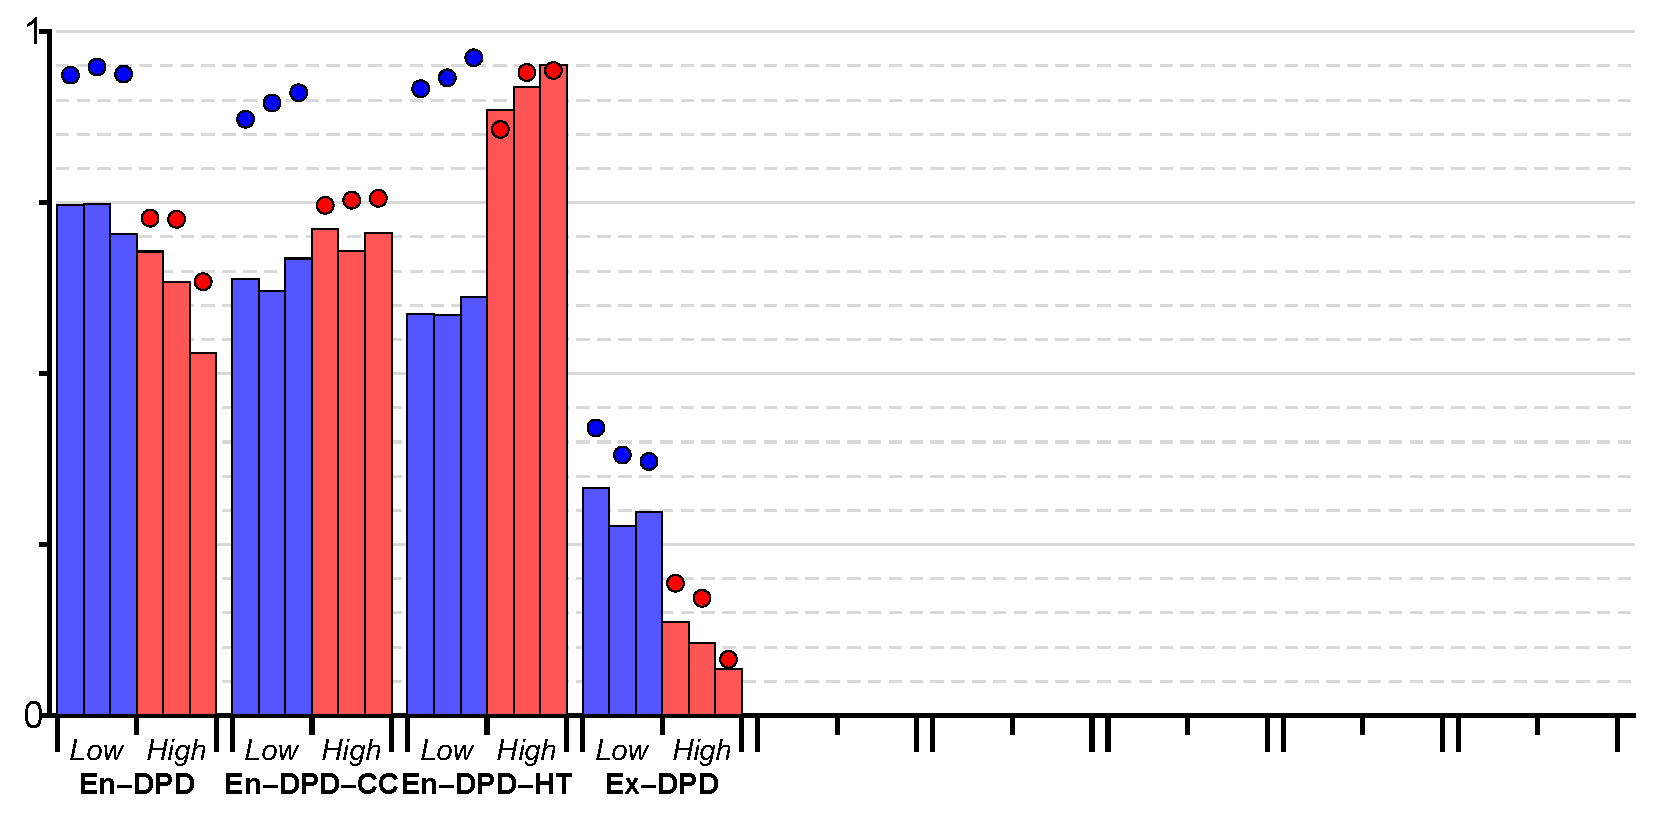
\includegraphics[width=1.0\textwidth]{./i/col_bar_StateCoop_block_ExDPD.pdf}
\end{center}
\end{card}
\end{frame}

\begin{frame}{Subject Cooperation:Ex-DPD }

\begin{card}
\begin{center}
	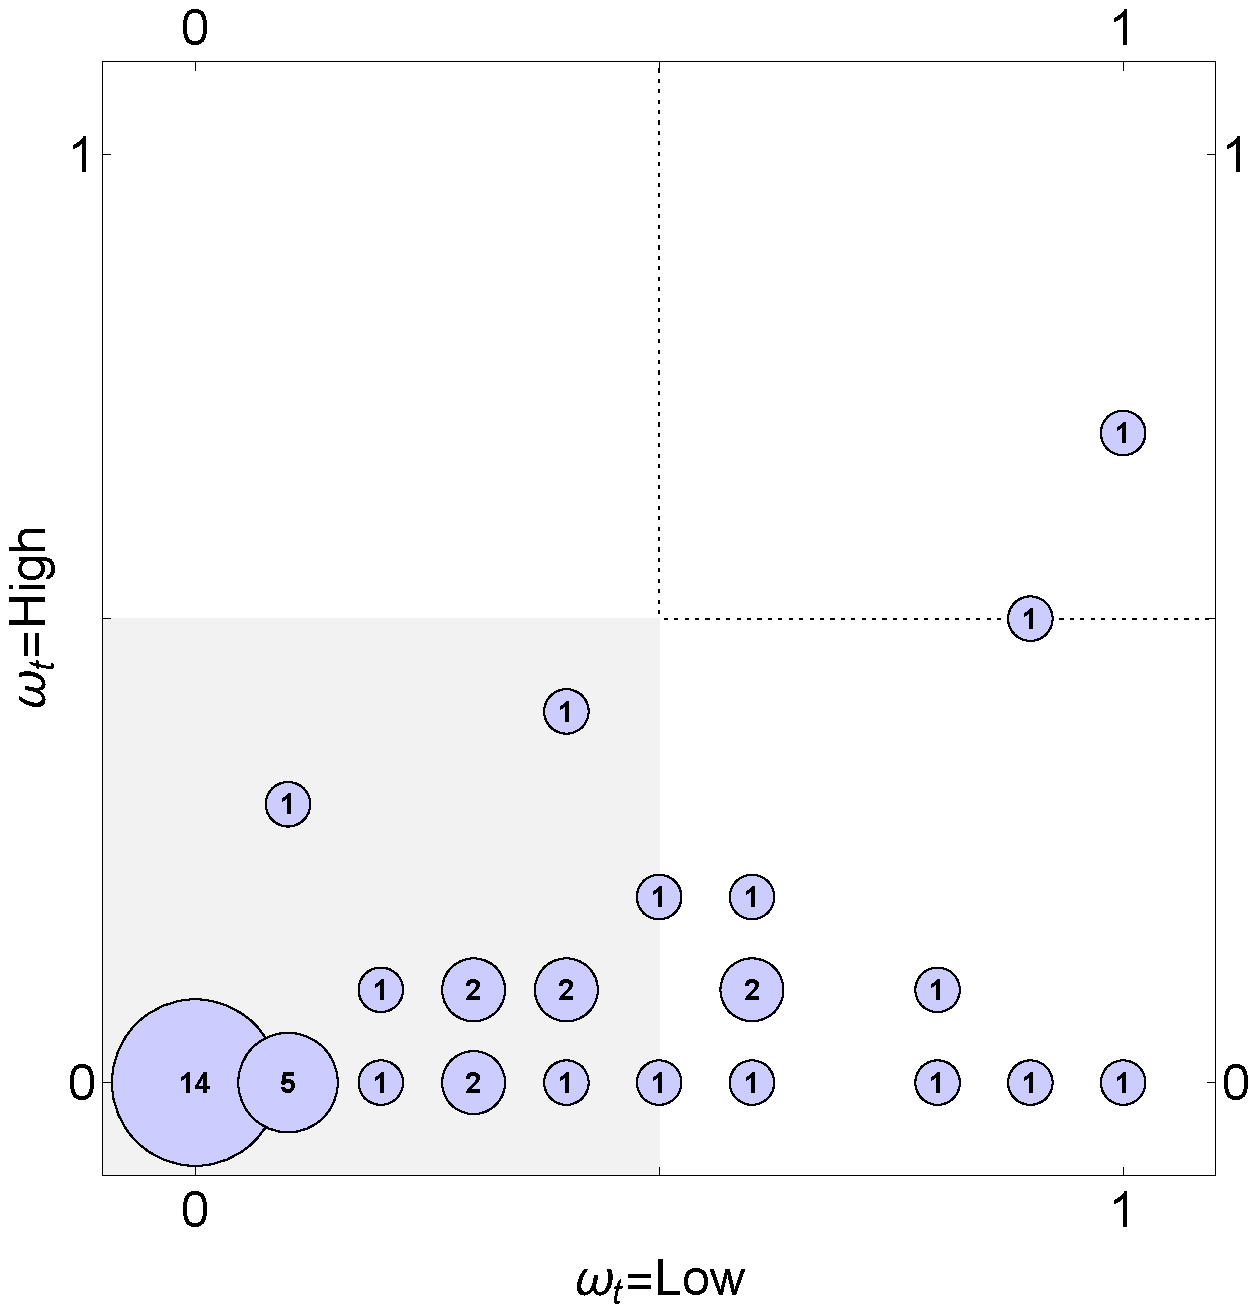
\includegraphics[width=0.6\textwidth]{./i/col_subject_stateCooperation_L5_ExDPD.pdf}
\end{center}
\end{card}
\end{frame}


\begin{frame}{Strategies (En-DPD$\rightarrow$Ex-DPD)}

\begin{card}
Popular pure strategy Markov:
\begin{itemize}
\item C-C: $7.9\%\rightarrow0.0\%$
\item C-D: $23.5\%\rightarrow7.3\%$
\item D-D (MPE): $4.7\%\rightarrow63.2\%$
\end{itemize}
\end{card}
\begin{card} 
Popular history-dependent strategies
\begin{itemize}
\item Grim trigger $13.8\%\rightarrow19.5\%$
\end{itemize}
\end{card}

\end{frame}

\begin{frame}

\begin{card}[Result 5]
Without the dynamic externality subjects cooperation falls
markedly
\end{card}
\end{frame}


\begin{frame}

\begin{card}
\begin{center}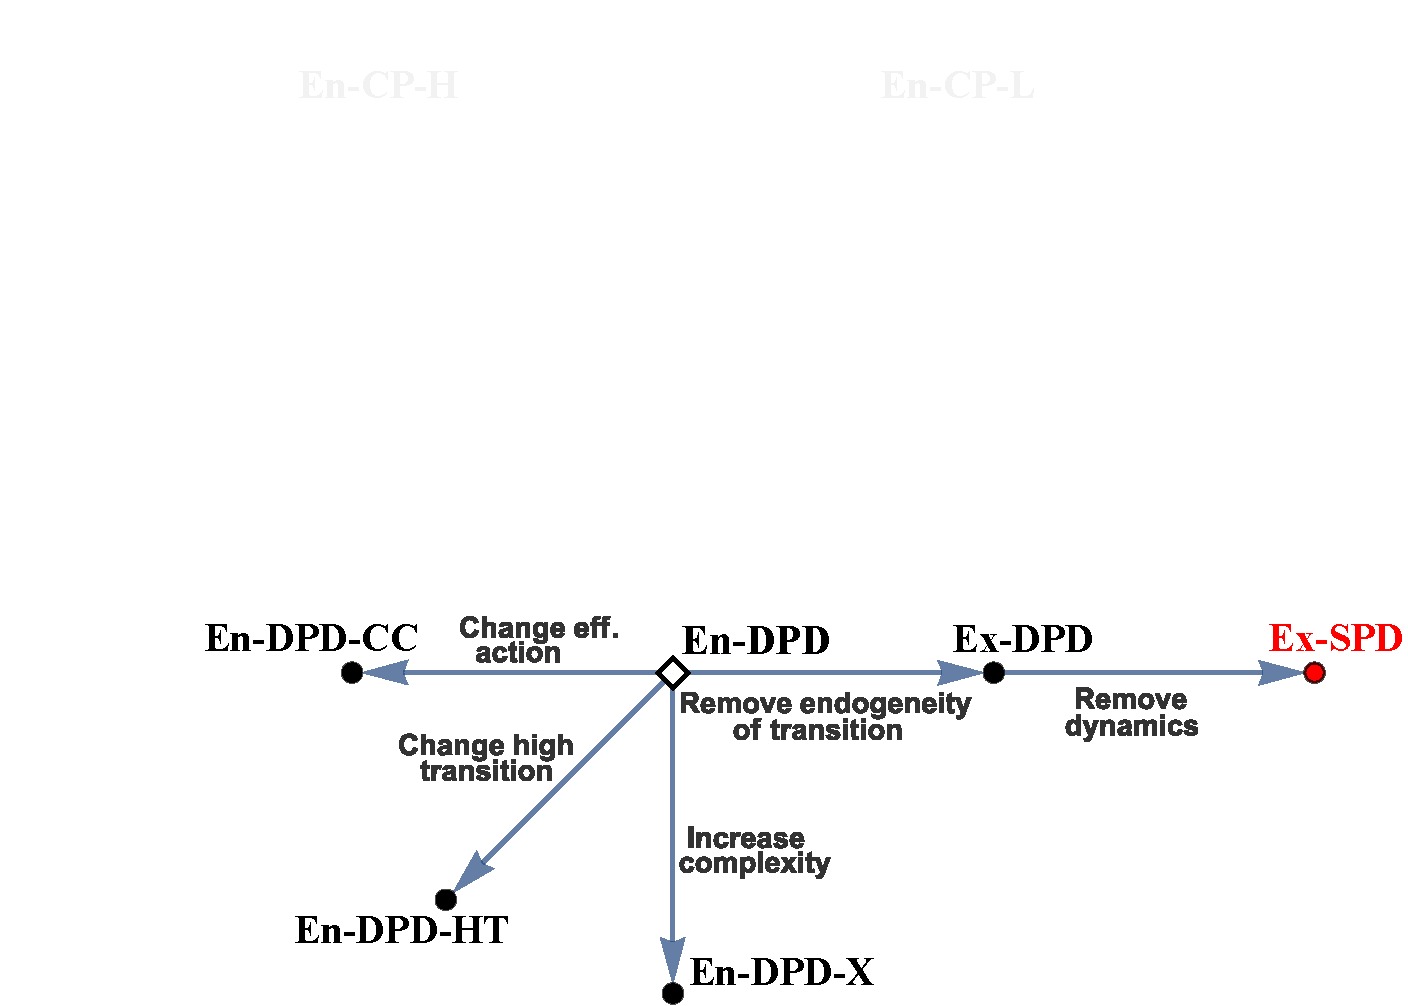
\includegraphics[height=0.7\textwidth]{./i/FlowChart6.pdf}
\end{center}
\end{card}
\end{frame}


\begin{frame}{En/Ex-DPD-2 $\rightarrow$ Ex-SPD-2}

\begin{card}
In our Dynamic-PD games, the state is changing over time

What is the effect in the Exog-DPD from the changing state?
\end{card}
\begin{card}[Manipulation 5] Remove dynamics within cycles:

    \begin{itemize}
    \item At the start of the game, randomly select either High or Low
    \item State tomorrow equals state today.
    \item Each cycle is an indefinitely repeated PD game
    \end{itemize}
\end{card}
\end{frame}

\begin{frame}{Results: Cooperation by State}
    \begin{card}
    \begin{center}
    	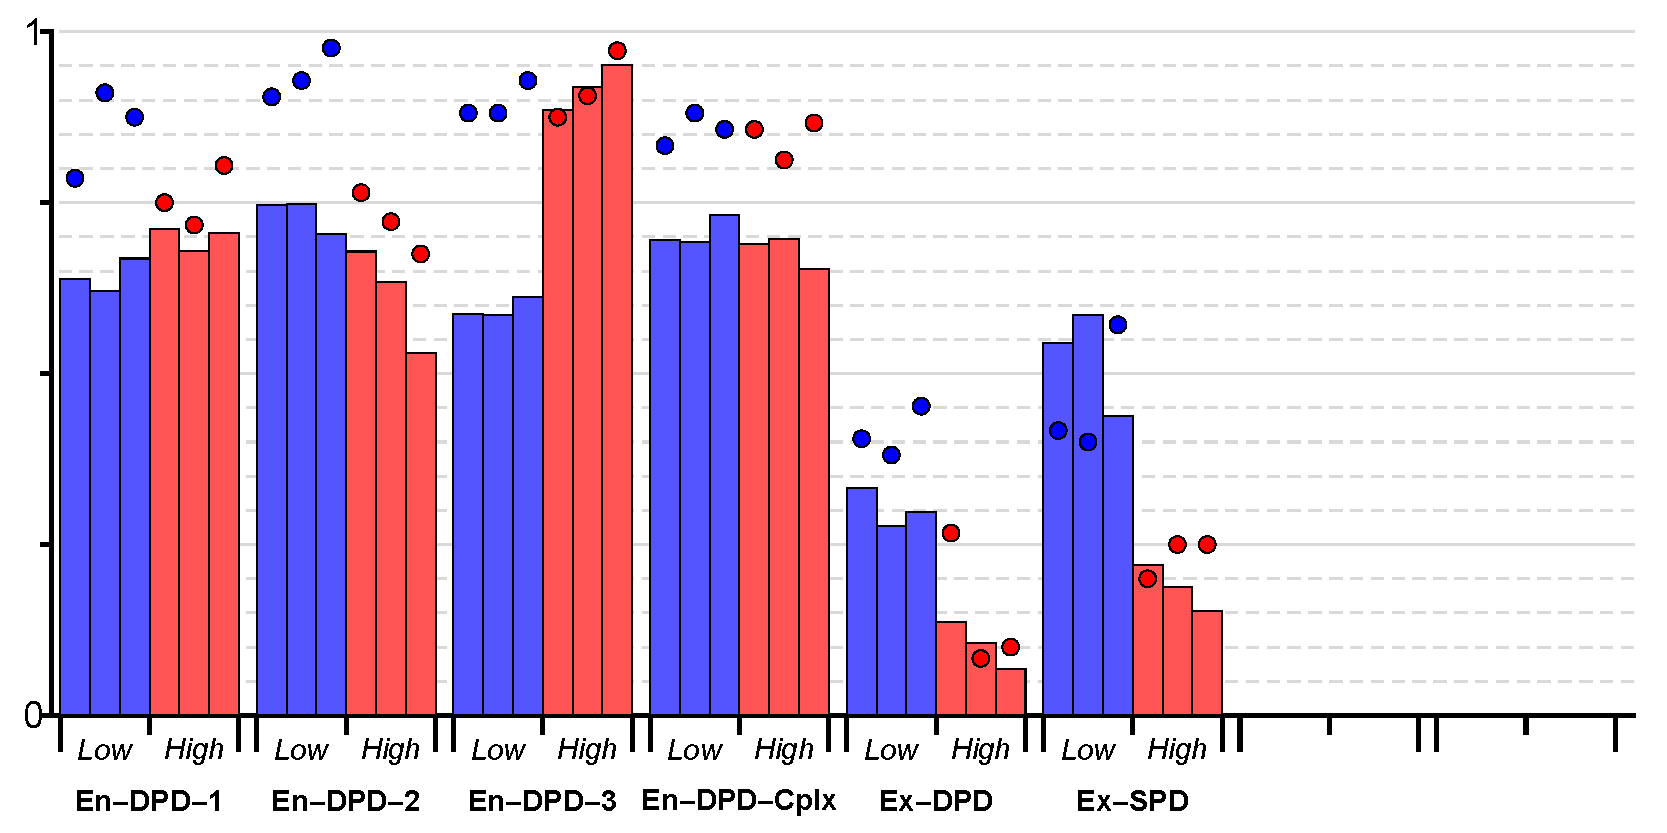
\includegraphics[width=1.0\textwidth]{./i/col_bar_StateCoop_block_ExIRPD.pdf}
    \end{center}
    \end{card}
\end{frame}

\begin{frame}{Subject Cooperation:Ex-DPD}
\begin{card}
\begin{center}
	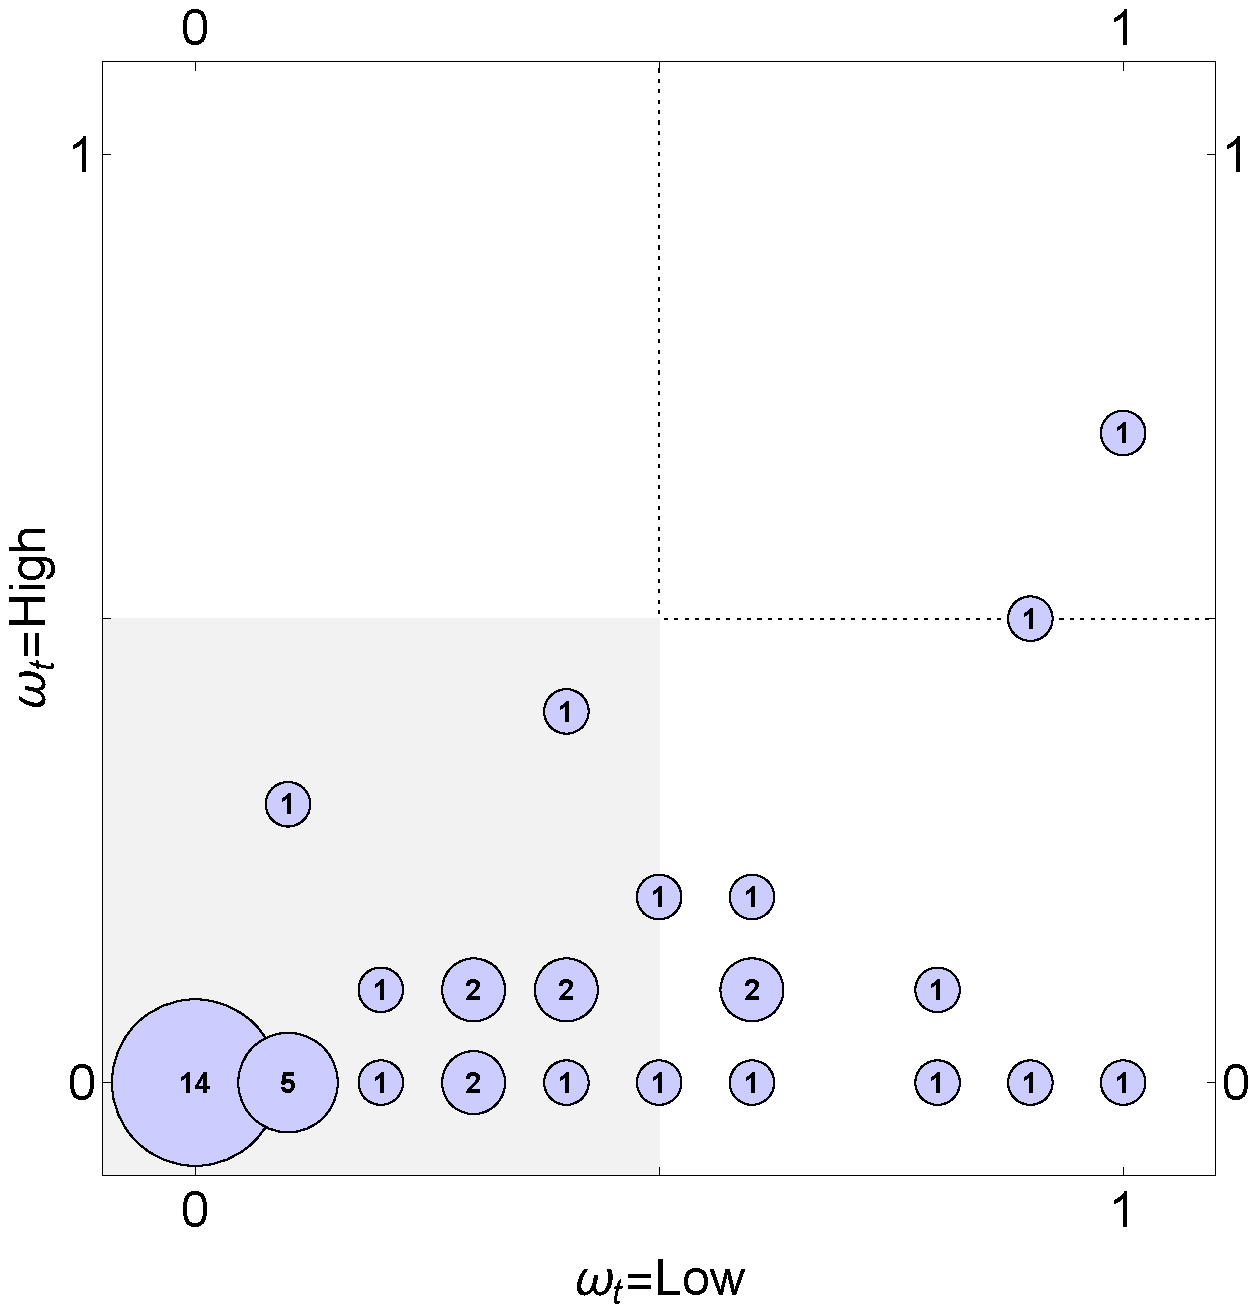
\includegraphics[width=0.6\textwidth]{./i/col_subject_stateCooperation_L5_ExDPD.pdf}
\end{center}
\end{card}
\end{frame}
\begin{frame}{Subject Cooperation:Ex-SPD}
\begin{card}
\begin{center}
	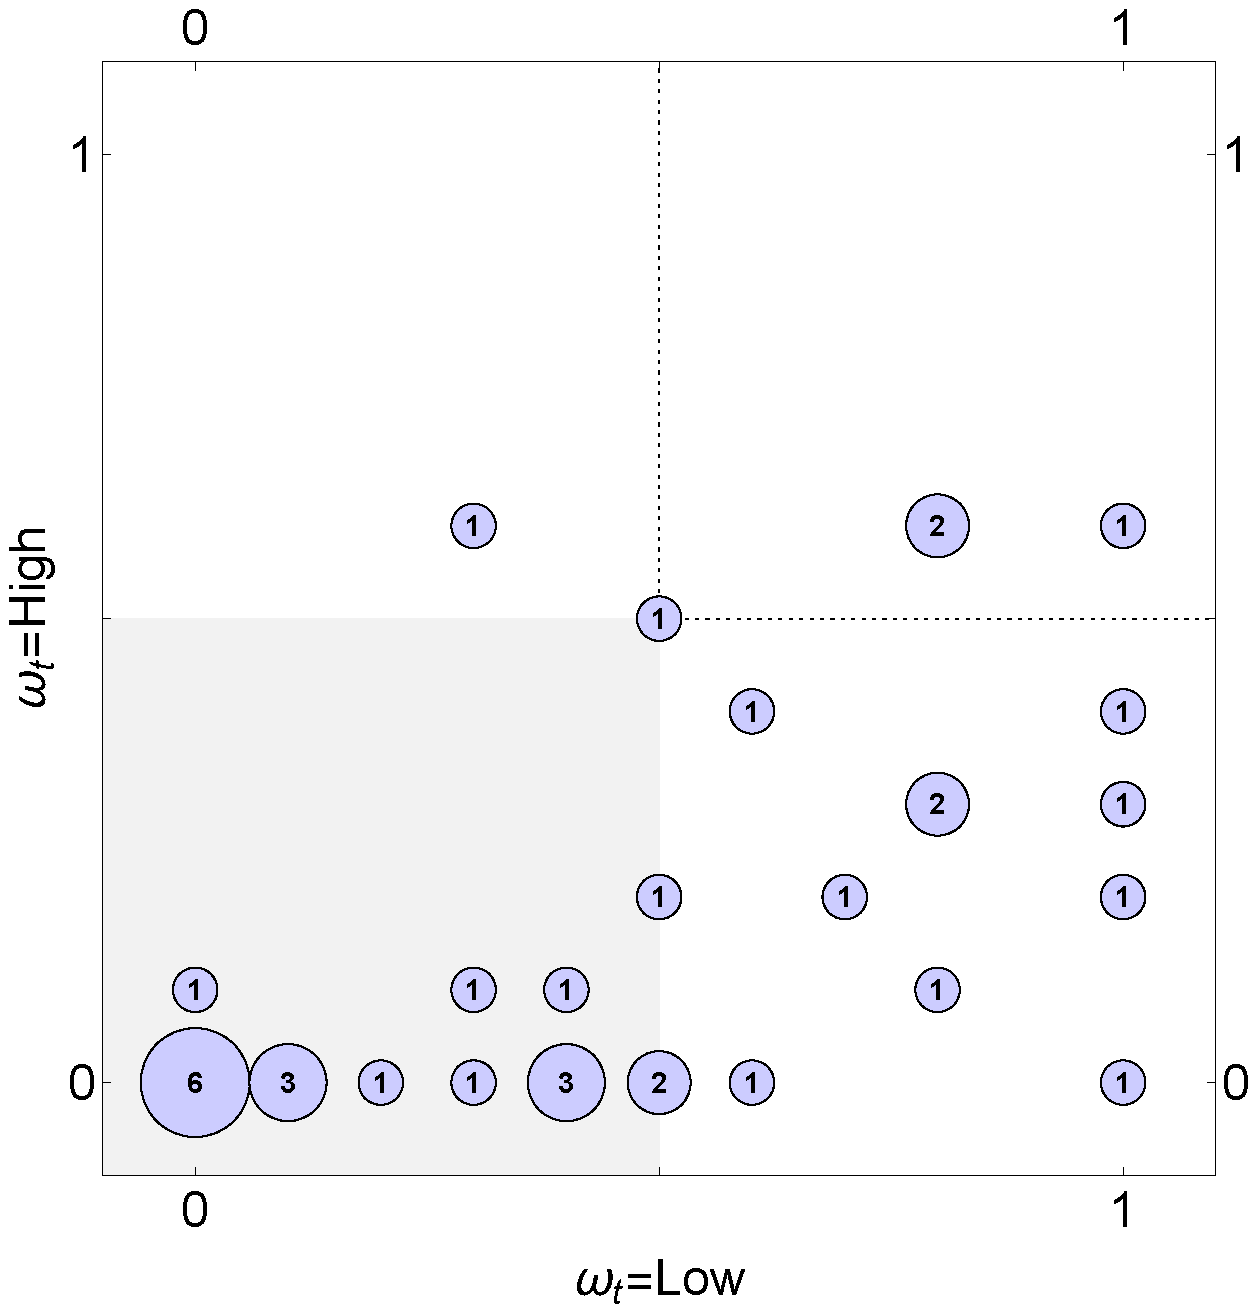
\includegraphics[width=0.6\textwidth]{./i/col_subject_stateCooperation_L5_ExIRPD.pdf}
\end{center}
\end{card}
\end{frame}

\begin{frame}{Strategies (Ex/En-DPD$\rightarrow$SPD)}

\begin{card}
 Cooperation rates at each state match behavior in each game:

\begin{itemize}
\item Low state, Grim is risk-dominant, observe more cooperation
\item High state, All-D is risk dominant, observe mostly defections
\end{itemize}
Removing the dynamics increases cooperation in the low state
\end{card}
\end{frame}

\begin{frame}
\begin{card}[Result 6]
Dynamically evolving (but exogenous) environments reduce conditional
cooperation
\end{card}
\end{frame}

\begin{frame}
\begin{card}
\begin{center}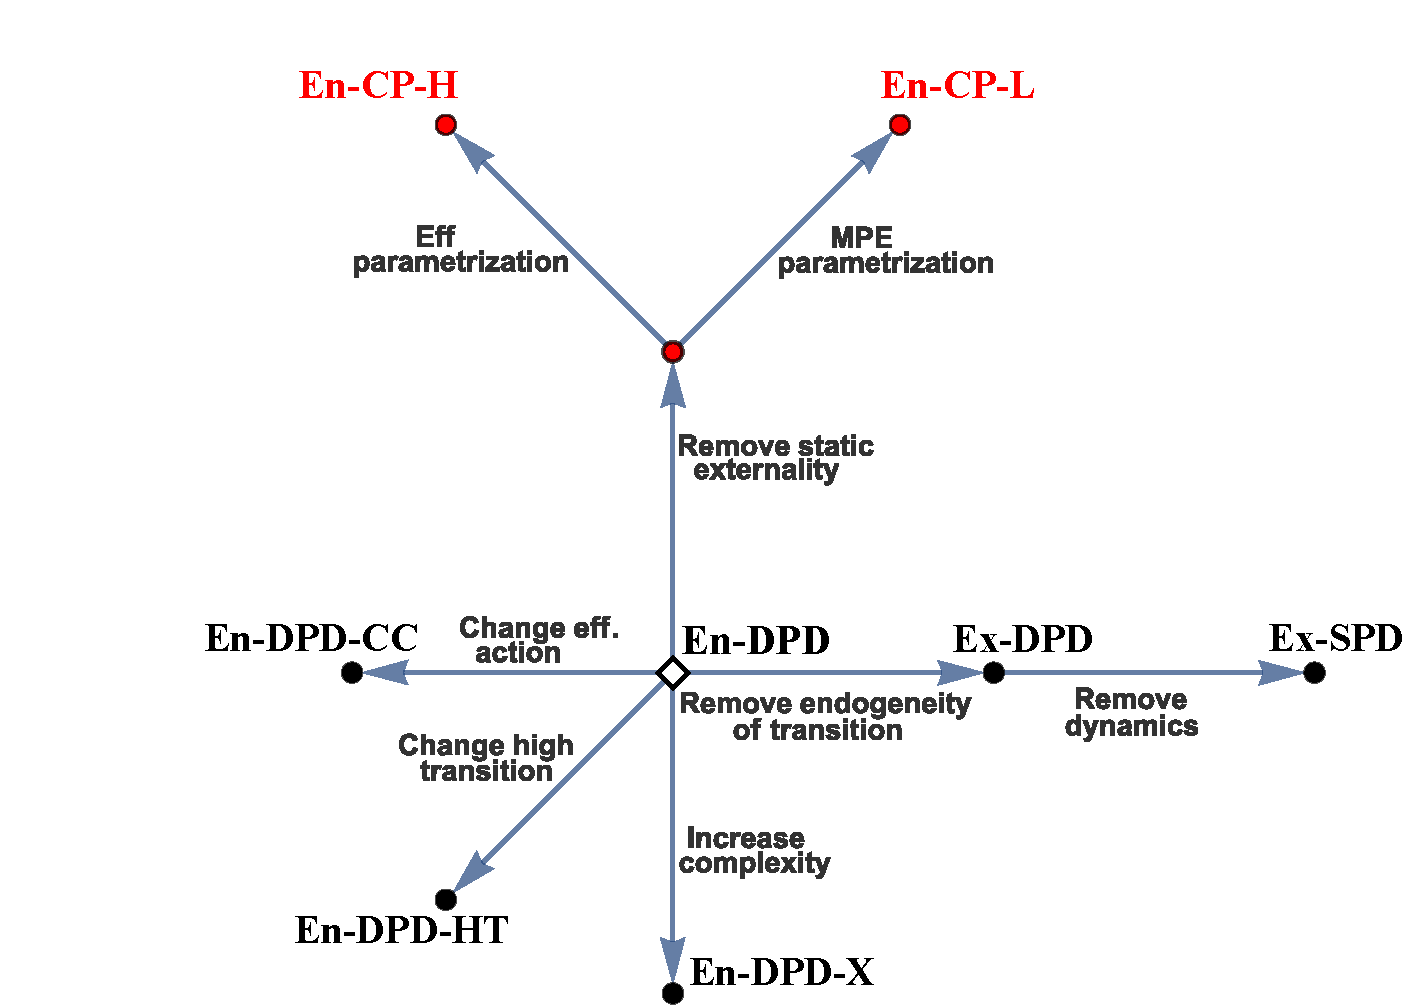
\includegraphics[height=0.7\textwidth]{./i/FlowChart7.pdf}
\end{center}
\end{card}
\end{frame}


\begin{frame}{En-DPD$\rightarrow$ En-CP}
\begin{card}
 In PD games, the action choice today has a static externality, my
action choice affects your payoff today

 We know that removing the dynamic externality reduces cooperation,
but what are the effects from removing the static externality?
\end{card}
\begin{card}[Manipulation 6 \& 7] Remove the static externalities:
\begin{itemize}
\item Same transition rule as En-DPD
\item Player 1's payoff today unaffected by Player 2's action today
\end{itemize}
\end{card}
\end{frame}
\begin{frame}{Common Pool-Low}
\begin{center}
\begin{table}
\centering{}\subfloat{\centering{}{\small{}}%
\begin{tabular}{ccP{0.1\textwidth}|P{0.1\textwidth}}
\multicolumn{4}{c}{\textcolor{red}{$\omega$=Low}}\\ 

 &  & \multicolumn{2}{c}{2}\\ 
 &  & \multicolumn{1}{P{0.1\textwidth}}{\textbf{C}} & D\\ 
\cline{3-4}
\multirow{2}{*}{1} & \multicolumn{1}{c|}{\textbf{C}} & \textbf{\textcolor{blue}{100}} & \multicolumn{1}{P{0.1\textwidth}|}{\textcolor{red}{100}}\\ 
\cline{3-4}
 & \multicolumn{1}{c|}{D} & \textcolor{red}{125} & \multicolumn{1}{P{0.1\textwidth}|}{\textcolor{red}{125}}\\ 
\cline{3-4}
\end{tabular}}\subfloat{\centering{}{\small{}}%
\begin{tabular}{ccP{0.1\textwidth}|P{0.1\textwidth}}
\multicolumn{4}{c}{\textcolor{blue}{$\omega$=High}}\\ 

 &  & \multicolumn{2}{c}{2}\\ 
 &  & \multicolumn{1}{P{0.1\textwidth}}{C} & \textbf{D}\\ 
\cline{3-4}
\multirow{2}{*}{1} & \multicolumn{1}{c|}{C} & \textcolor{blue}{130} & \multicolumn{1}{P{0.1\textwidth}|}{\textcolor{blue}{130}}\\ 
\cline{3-4}
 & \multicolumn{1}{c|}{\textbf{D}} & \textcolor{blue}{190} & \multicolumn{1}{P{0.1\textwidth}|}{\textbf{\textcolor{red}{190}}}\\ 
\cline{3-4}
\end{tabular}}
\end{table}

\end{center}
\begin{card}
\begin{itemize}
    \item Same state transition rule as En-DPD, same symmetric Markov
    \item Removes contemporaneous externality
    \item Same MPE as En-DPD, $C$ in Low, $D$ in High
\end{itemize}
\end{card}
\end{frame}

\begin{frame}{Common Pool-High}
\begin{center}
\begin{table}
\centering{}\subfloat{\centering{}{\small{}}%
\begin{tabular}{ccP{0.1\textwidth}|P{0.1\textwidth}}
\multicolumn{4}{c}{\textcolor{red}{$\omega$=Low}}\\ 

 &  & \multicolumn{2}{c}{2}\\ 
 &  & \multicolumn{1}{P{0.1\textwidth}}{\textbf{C}} & D\\ 
\cline{3-4}
\multirow{2}{*}{1} & \multicolumn{1}{c|}{\textbf{C}} & \textcolor{blue}{100} & \multicolumn{1}{P{0.1\textwidth}|}{\textcolor{red}{100}}\\ 
\cline{3-4}
 & \multicolumn{1}{c|}{D} & \textcolor{red}{125} & \multicolumn{1}{P{0.1\textwidth}|}{\textcolor{red}{125}}\\ 
\cline{3-4}
\end{tabular}}\subfloat{\centering{}{\small{}}%
\begin{tabular}{rcP{0.1\textwidth}|P{0.1\textwidth}}
\multicolumn{4}{c}{\textcolor{blue}{$\omega$=High}}\\ 

 &  & \multicolumn{2}{c}{2:}\\ 
 &  & \multicolumn{1}{P{0.1\textwidth}}{C} & \textbf{D}\\ 
\cline{3-4}
\multirow{2}{*}{1:} & \multicolumn{1}{c|}{C} & \textcolor{blue}{130} & \multicolumn{1}{P{0.1\textwidth}|}{\textcolor{blue}{130}}\\ 
\cline{3-4}
 & \multicolumn{1}{c|}{\textbf{D}} & \textcolor{blue}{280} & \multicolumn{1}{P{0.1\textwidth}|}{\textbf{\textcolor{red}{280}}}\\ 
\cline{3-4}
\end{tabular}}
\end{table}
\end{center}
\begin{card}
\begin{itemize}
\item Payoffs are calibrated so that period tensions are the same for alternation
between $(C,D)$ and $(D,C)$ in En-DPD
\item Same Efficient frontier as the DPD-game
\end{itemize}
\end{card}
\end{frame}


\begin{frame}{Results: Cooperation by State}
\begin{card}
\begin{center}
	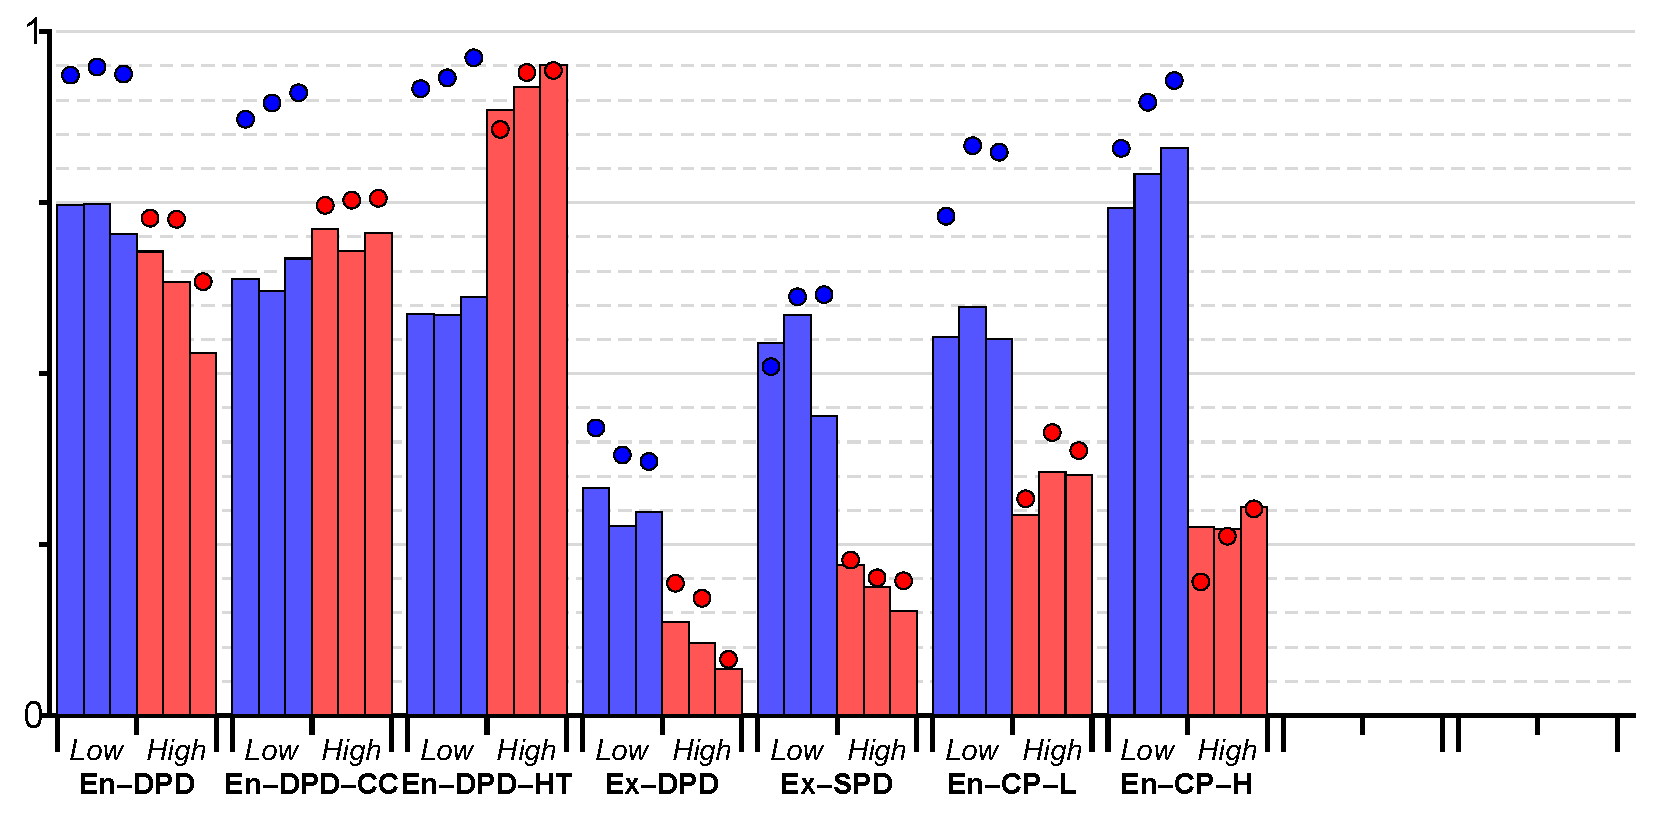
\includegraphics[width=1.0\textwidth]{./i/col_bar_StateCoop_block_CP_H.pdf}
\end{center}
\end{card}
\end{frame}
\begin{frame}{Subject Cooperation: En-DPD}
\begin{card}
\begin{center}
	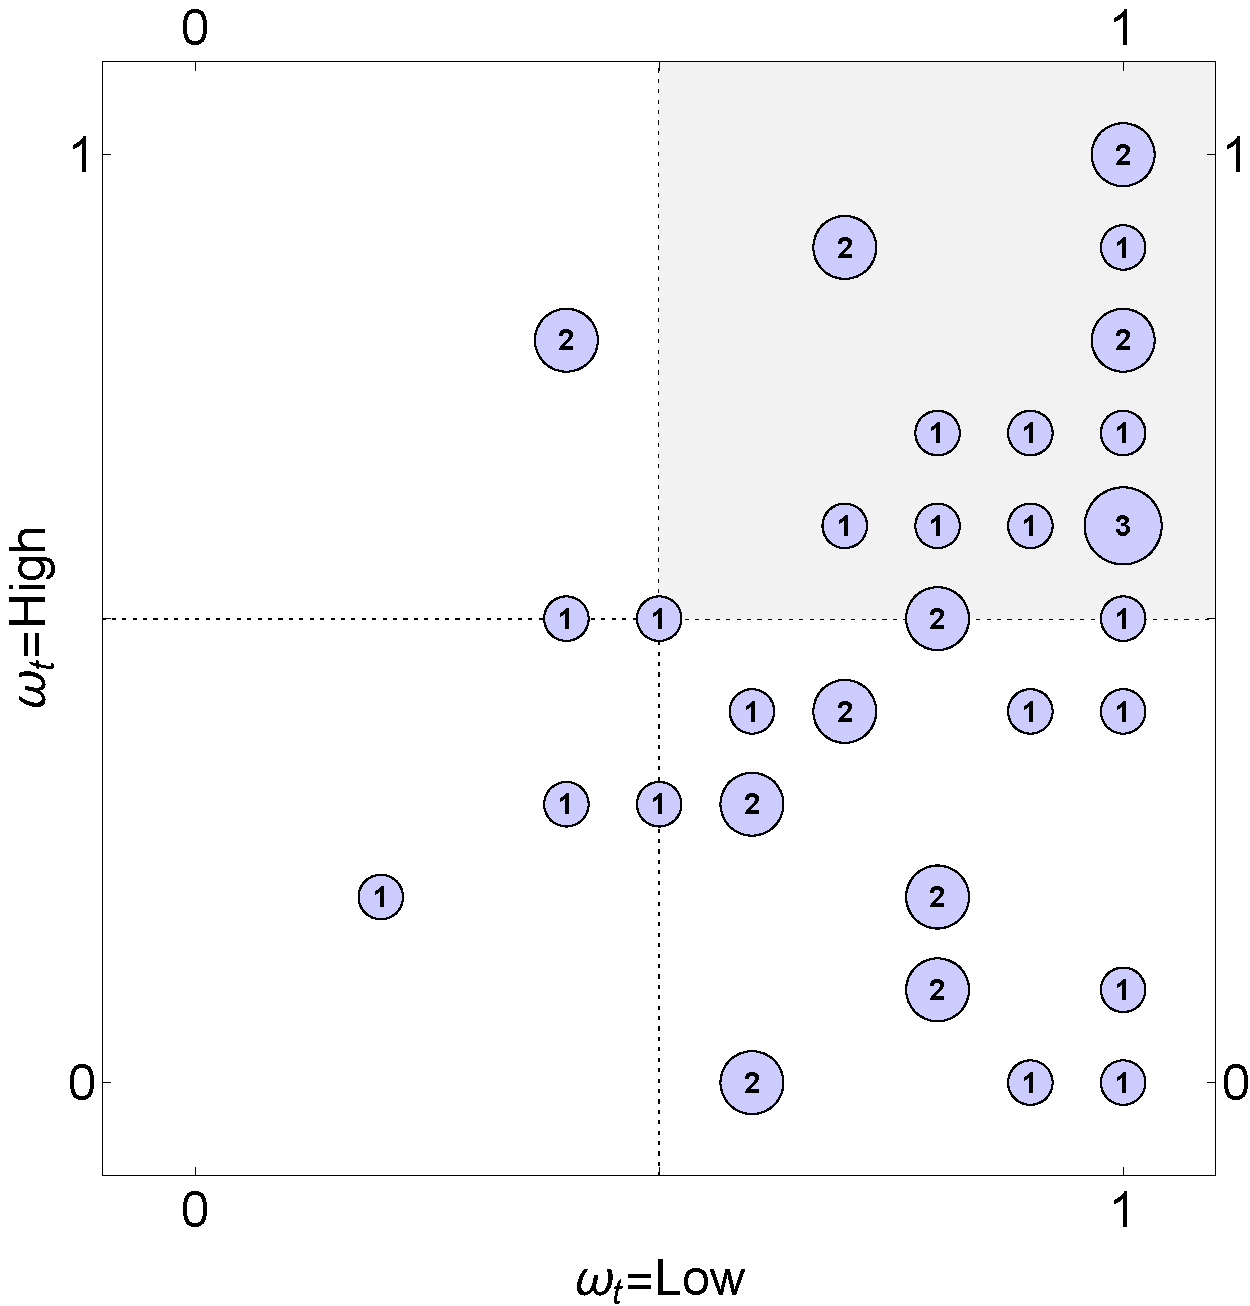
\includegraphics[width=0.6\textwidth]{./i/col_subject_stateCooperation_L5_EnDPD_2.pdf}
\end{center}
\end{card}
\end{frame}
\begin{frame}{Subject Cooperation: En-CP-L }
\begin{card}
\begin{center}
	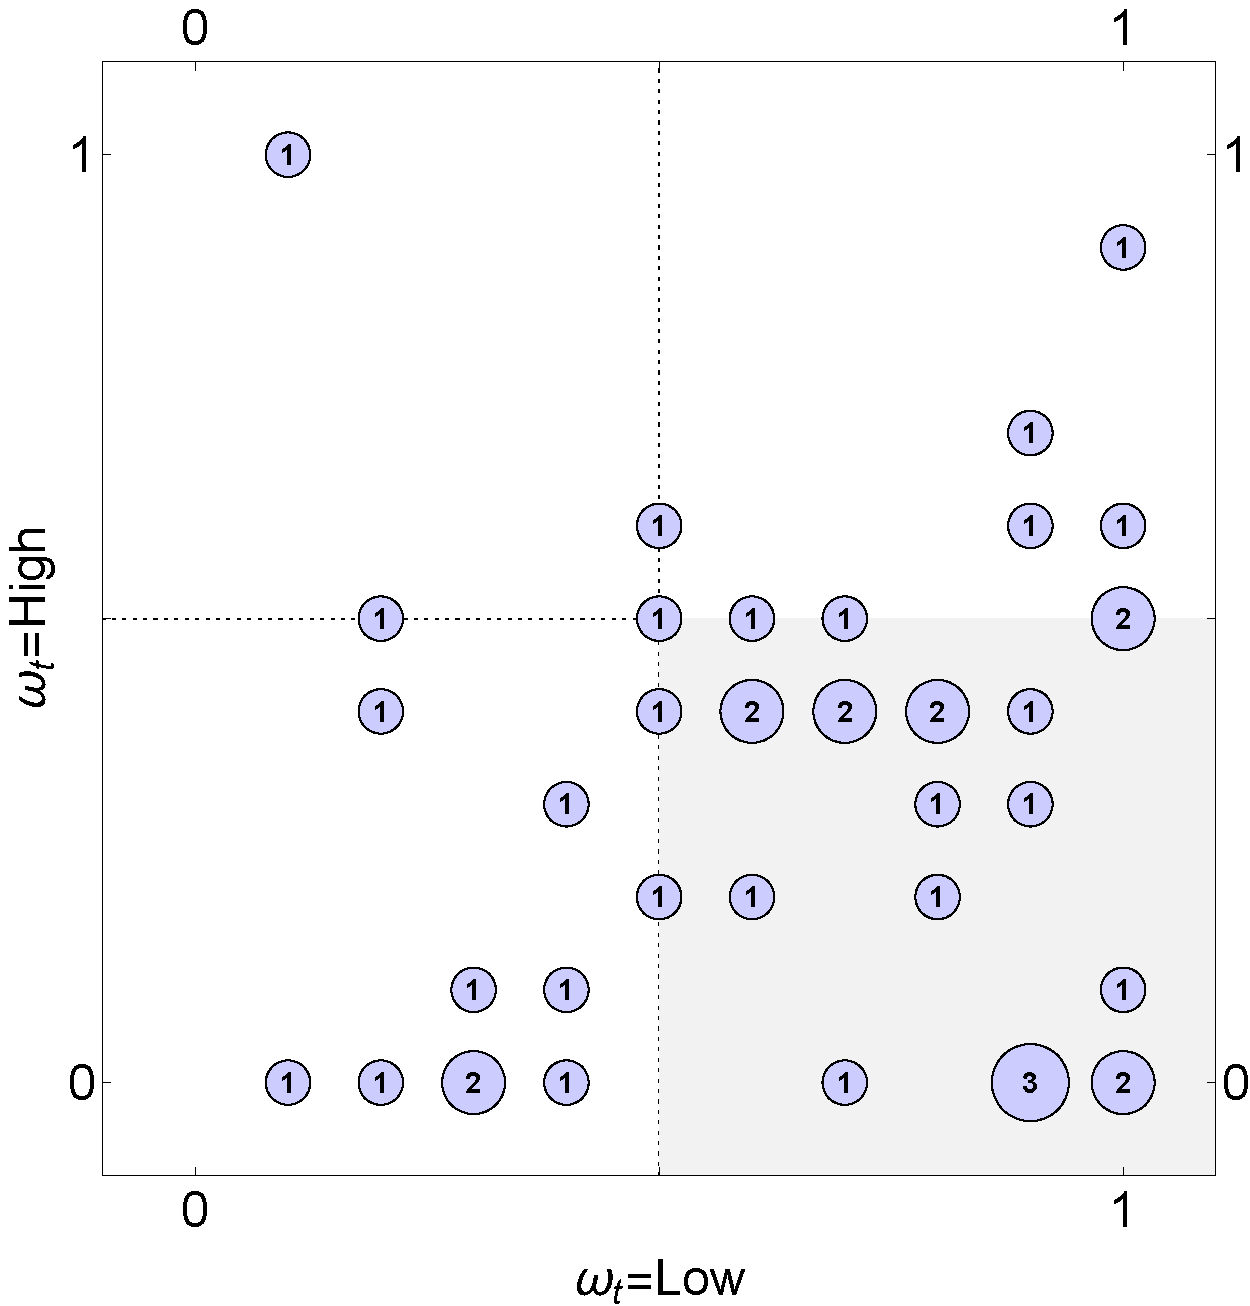
\includegraphics[width=0.6\textwidth]{./i/col_subject_stateCooperation_L5_CP_L.pdf}
\end{center}
\end{card}
\end{frame}
\begin{frame}{Subject Cooperation: En-CP-H }
\begin{card}
\begin{center}
	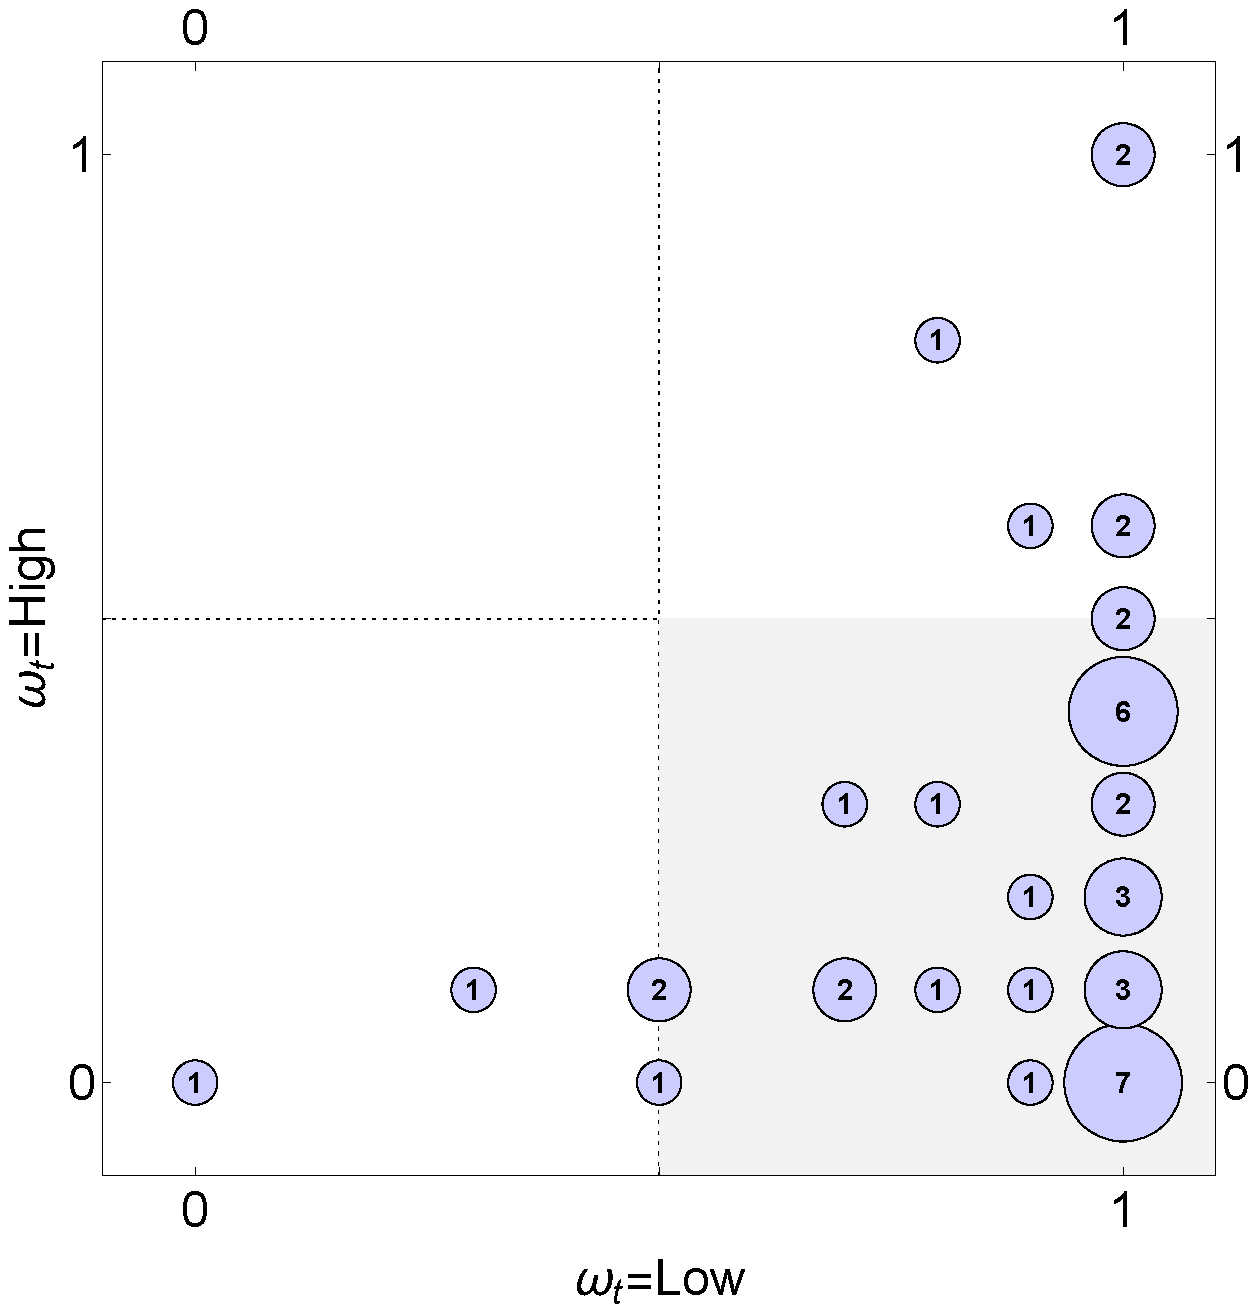
\includegraphics[width=0.6\textwidth]{./i/col_subject_stateCooperation_L5_CP_H.pdf}
\end{center}
\end{card}
\end{frame}

\begin{frame}{Strategies (En-DPD$\rightarrow$En-CP-L$\rightarrow$En-CP-H)}
\begin{card}
 Markov strategies
\begin{itemize}
\item C-C: $7.9\%\rightarrow6.8\%\rightarrow7.8\%$
\item \textbf{C-D:} $23.5\%\rightarrow23.9\%\rightarrow35.4\%$
\item \textbf{D-D:} $4.7\%\rightarrow12.3\%\rightarrow4.8\%$
\end{itemize}
\end{card}
\begin{card} Popular history-dependent strategies

\begin{itemize}
\item Grim trigger $11.4\%\rightarrow7.3\%\rightarrow0.0\%$
\item D-Alternate, D-trigger $4.3\%\rightarrow16.1\%\rightarrow4.6\%$
\item C-Alternate, MPE-trigger $23.4\%\rightarrow9.1\%\rightarrow16.1\%$
\item D-Alternate, MPE-trigger $2.5\%\rightarrow17.2\%\rightarrow31.4\%$
\end{itemize}
\end{card}
\end{frame}
\begin{frame}
\begin{card}[Result 7]
Removing the static externalities, outcomes looks like it does generate greater coordination on the
MPE\end{card}
\end{frame}


\begin{frame}{Selection Index}
\begin{card}
 In repeated games, a large body of experimental work has shown that
the basin attraction helps predict equilibrium selection
\end{card}
\begin{card}
\centering 
{\small{}}%
\begin{tabular}{cc|P{0.18\textwidth}|P{0.18\textwidth}|}
 & \multicolumn{1}{c}{} & \multicolumn{2}{c}{Col:}\\ 
 & \multicolumn{1}{c}{} & \multicolumn{1}{P{0.18\textwidth}}{\textbf{Grim}} & \multicolumn{1}{P{0.18\textwidth}}{\textbf{All-D}}\\ 
\cline{3-4}
\multirow{2}{*}{Row:} & \textbf{Grim} & \textcolor{black}{$1$} & -$S(\delta)$\\ 
\cline{3-4}
 & \textbf{All-D} & $T(\delta)$ & \textcolor{black}{$0$}\\ 
\cline{3-4}
\end{tabular}
\end{card}
\end{frame}

\begin{frame}{Selection Index}
\begin{card}
\centering
{\small{}}%
\begin{tabular}{cc|P{0.18\textwidth}|P{0.18\textwidth}|}
 & \multicolumn{1}{c}{} & \multicolumn{2}{c}{Col:}\\ 
 & \multicolumn{1}{c}{} & \multicolumn{1}{P{0.18\textwidth}}{\textbf{Grim}} & \multicolumn{1}{P{0.18\textwidth}}{\textbf{All-D}}\\ 
\cline{3-4}
\multirow{2}{*}{Row:} & \textbf{Grim} & \textcolor{black}{$1$} & -$S(\delta)$\\ 
\cline{3-4}
 & \textbf{All-D} & $T(\delta)$ & \textcolor{black}{$0$}\\ 
\cline{3-4}
\end{tabular}
\end{card}
\begin{card}
Try to generalize this for the dynamic game
\begin{itemize}
    \item Replace All-D with the MPE
    \item Replace Grim with Efficient coperation on a MPE trigger
\end{itemize}
\end{card}
\end{frame}

\begin{frame}{Selection Index}
\begin{card}

\centering 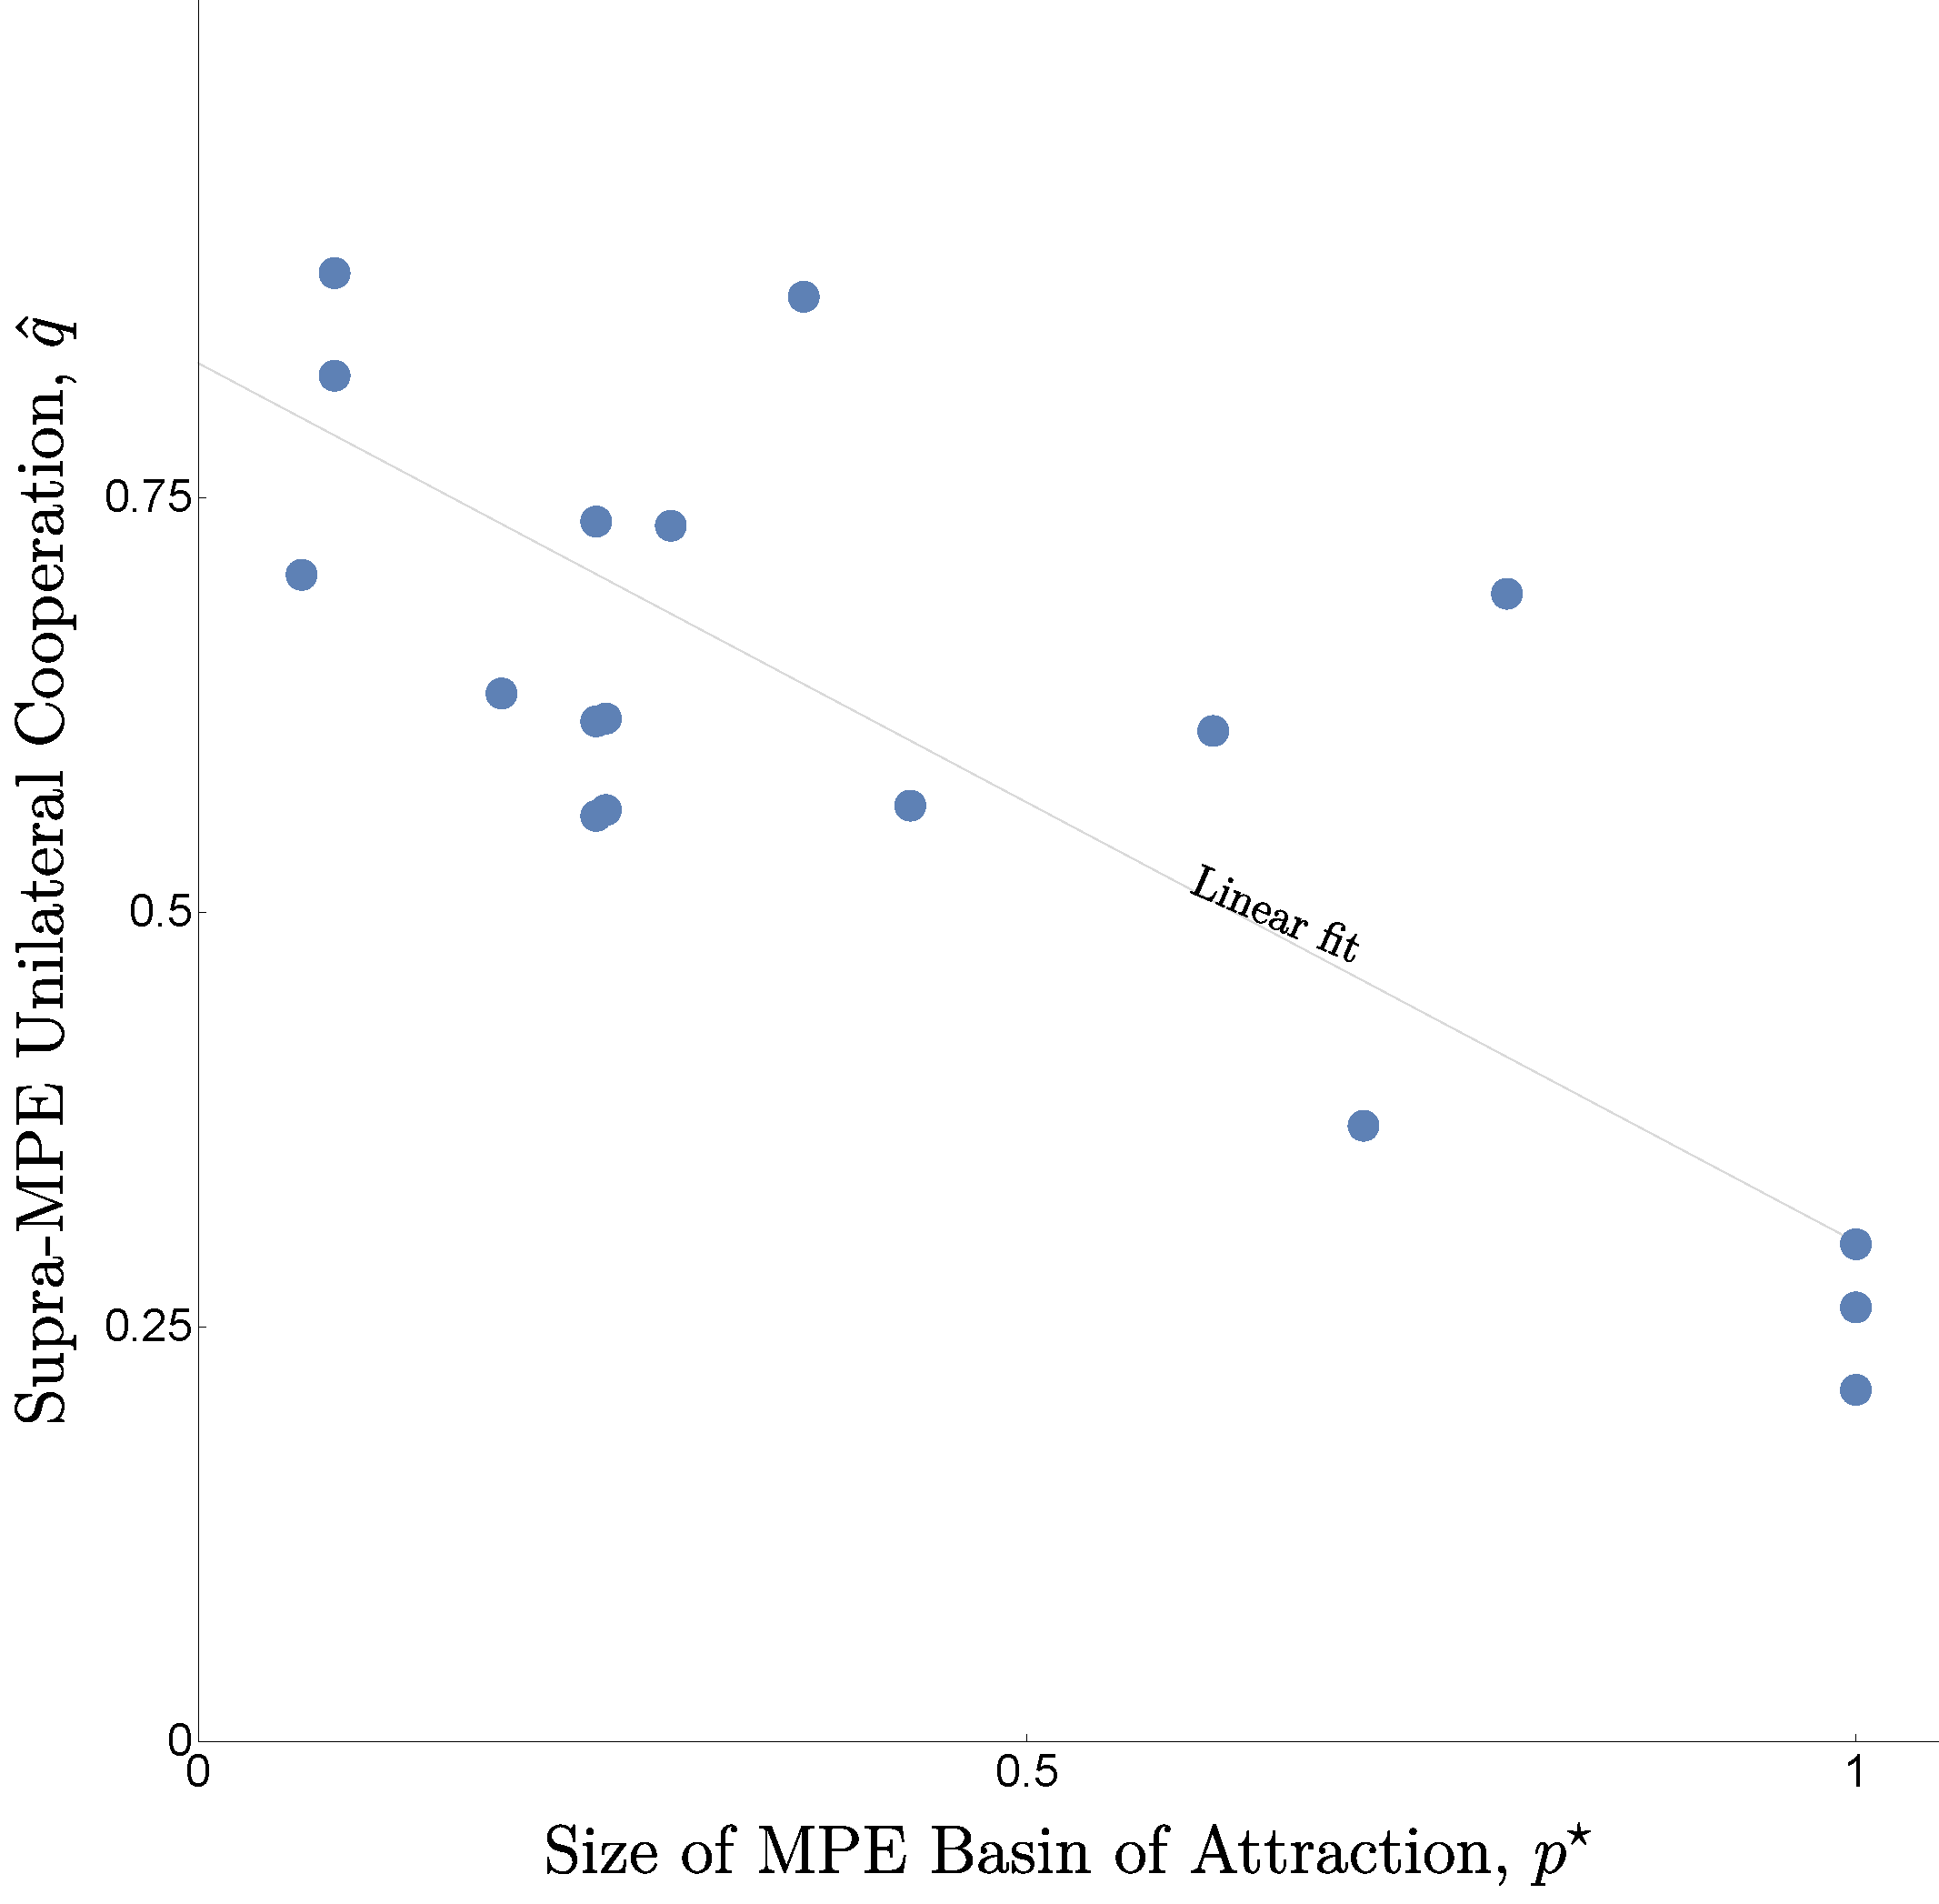
\includegraphics[width=0.7\textwidth]{./i/AlistairNew_Unilateral_2.pdf}
\end{card}
\end{frame}

\end{document}

